\documentclass[11pt]{article}

% Begin preamble.tex
\usepackage[T1]{fontenc}
\usepackage[utf8]{inputenc}
\usepackage{lmodern}
\usepackage[margin=1in]{geometry}
\usepackage{amsmath,amssymb,amsthm,mathtools}
\usepackage{microtype,booktabs,array,longtable,enumitem}
\usepackage{xcolor,tikz}
\usetikzlibrary{arrows.meta,positioning,calc}
\definecolor{linkblue}{RGB}{30,67,108}
\usepackage[colorlinks=true,linkcolor=linkblue,citecolor=linkblue,urlcolor=linkblue,
  pdftitle={Spatial Compilation of Stochastic Chemical Trajectories},
  pdfauthor={Harjas Sandhu}]{hyperref}
\usepackage[nameinlink,noabbrev]{cleveref}
\usepackage{fancyhdr}
\pagestyle{fancy}\fancyhf{}
\fancyhead[L]{\small Spatial compilation of chemical trajectories}
\fancyhead[R]{\small H. Sandhu}\fancyfoot[C]{\thepage}
\setlength{\headheight}{14pt}
\setlength{\emergencystretch}{2em}
\setlist{itemsep=3pt,topsep=5pt}
\numberwithin{equation}{section}
\newtheorem{theorem}{Theorem}[section]
\newtheorem{lemma}[theorem]{Lemma}
\newtheorem{proposition}[theorem]{Proposition}
\newtheorem{corollary}[theorem]{Corollary}
\theoremstyle{definition}
\newtheorem{definition}[theorem]{Definition}
\newtheorem{example}[theorem]{Example}
\theoremstyle{remark}\newtheorem{remark}[theorem]{Remark}
\newcommand{\N}{\mathbb N}
\newcommand{\R}{\mathbb R}
\newcommand{\E}{\mathbb E}
\newcommand{\Prob}{\mathbb P}
\newcommand{\TV}{d_{\mathrm{TV}}}
\newcommand{\Var}{\operatorname{Var}}
\newcommand{\Lip}{\operatorname{Lip}}
\newcommand{\Vol}{\operatorname{Vol}}
\newcommand{\diag}{\operatorname{diag}}
\newcommand{\tr}{\operatorname{tr}}
\newcommand{\supp}{\operatorname{supp}}
\newcommand{\dist}{\operatorname{dist}}
\newcommand{\Unif}{\operatorname{Unif}}
\newcommand{\K}{\mathcal K}
\newcommand{\cE}{\mathcal E}
\newcommand{\Ff}{F_{\mathrm{all}}}
\newcommand{\Rnum}{R_{\mathrm{num}}}
\newcommand{\ind}{\mathbf 1}
\newcommand{\dt}{\,dt}
\newcommand{\ds}{\,ds}
\newcommand{\dd}{\,d}
\newcommand{\pa}[1]{\left(#1\right)}
\newcommand{\abs}[1]{\left|#1\right|}
\newcommand{\norm}[1]{\left\|#1\right\|}
\DeclareMathOperator*{\argmin}{arg\,min}
\title{Spatial Compilation of\\Stochastic Chemical Trajectories}
\author{Harjas Sandhu\\[3pt]\small The University of Queensland\\
\small\href{mailto:harjas.sandhu@student.uq.edu.au}{harjas.sandhu@student.uq.edu.au}}
\date{13 November 2026}

% End preamble.tex

\begin{document}
\maketitle
\begin{abstract}
A well-mixed reaction specification does not by itself determine a local
particle implementation. We construct such an implementation for finite
labelled mass-action networks with a positive integer conservation law,
a supplied reverse involution and prescribed rational detailed-balanced
activities. The compiler produces elementary reactions, strictly positive
particle radii, constant rational coefficients, a payload decoder and one
known slowdown. From every feasible initial placement, including simultaneous
contacts, the decoded timed and labelled path approximates the target path
in total variation. Transport may be unknown, spatially inhomogeneous and
time dependent; the estimate permits full-history predictable chemical,
drift and correlated covariance faults within a computed tolerance. A dilute
hard-ball Poincar\'e inequality, proved by buffering, rank separation and
one-particle coordinate paths, supplies the required population-uniform
polynomial mixing estimates. We account for duration, inverse radii and
coefficients, precision, every attempted reaction and the actual wall and
pair pushes. The bounds are polynomial in a stated numerical charge together
with the binary input length. They allow severe dilution and slowdown and
concern an ideal particle model, without asserting a molecular realization
or a practical advantage.
\end{abstract}
\makeatletter
{\small\setcounter{tocdepth}{1}
\renewcommand*\l@section[2]{\@dottedtocline{1}{0pt}{1.8em}{#1}{#2}}
\tableofcontents}
\makeatother
\clearpage

% Begin sections/01_introduction.tex
\section{From a reaction specification to moving particles}
\label{sec:intro}

A mass-action model specifies counts and reaction events while suppressing
positions, encounter delays and rejected product placements. Can such a table
be compiled into a local particle system that reproduces the full stochastic
record, with one known change of clock and explicit resource bounds?

Here the target is finite, conservative and reversible; its reaction order,
species and labels may vary. The vessel is a three-dimensional rational
convex polytope and every particle has positive radius. The compiler uses
bounds on unknown species-dependent transport and predictable perturbations,
without measuring initial positions or solving a configuration-space equation.

Accuracy concerns the joint law of initial counts, continuous firing times,
original labels and post-event counts, including null events. Total variation
therefore controls every measurable question about this finite-horizon record,
rather than just a single-time distribution. The clock change is deterministic;
no internal waiting time is removed. The path laws are approximated, not equal.

\paragraph{Contribution and relation to the kinetic companion.}
The elementary well-mixed compiler in \cite[Theorem~9.1]{Sandhu2026} is a
separate conservative, detailed-balanced construction. We use precisely that
theorem, with a smaller error budget. Its general open-network theorem has
a different input class and does not supply detailed balance. Our additional
operation is a finite-radius continuum realization with quantitative control
of transport, spatial rejection and the complete marked path. The central
geometric estimate is
\[
 \Var_{\mu_\K} f\le 2^{20}(1+N)\int_\K|\nabla f|^2\dd\mu_\K,
\]
for every labelled configuration space beneath the conserved cap, when the
computed radius is sufficiently small. Its proof avoids exponential
congestion in the number of particles. Local reflected estimates then give
all-start mixing and conditional comparison under history-dependent faults.
Finally, a category coupling preserves the actual hidden history while
matching the exact proposal times.

\paragraph{Predecessors.}
Programmable DNA controllers have experimental realizations with measured
performance \cite{Chen2013}. We instead specify an ideal stochastic model.
Elimination of fast intermediates is established:
Hoessly--Wiuf~\cite[Assumption~2 and Theorem~4.1]{HW2021} give a
finite-closed-set reduction controlling compact-time state probabilities.
That statement alone does not provide the full marked-path and resource
contract used here. Poisson product-form laws and their restrictions to
chemical classes are classical under appropriate balance hypotheses
\cite[Theorem~4.1 and Section~4.2]{ACK2010}.

Spatial detailed balance depends on placement as well as reaction rates.
Zhang--Isaacson~\cite[Section~III and Theorem~III.1]{ZI2022} give the relevant
forward/reverse flux criterion for reversible particle reactions, including
boundary effects. We apply it with anchored placement and steric rejection.
For reflected hard particles and contact-clock decomposition, see
Fradon~\cite[Theorem~2.2 and Proposition~3.4]{Fradon2009}. Its normal-reflection
theorems are not invoked as a theorem about arbitrary variable conormal
reflection. We supply that passage for the present geometry.
The smooth-boundary derivative formula used for local smoothing is
Cheng--Zhang~\cite[Theorem~2.5]{CZ2017}, with its curvature and local-time
hypotheses checked in \cref{app:imports}.

The contribution combines these components with the dilute hard-ball
comparison, conditional robustness and acyclic parameter choices needed for
a variable-network compiler. Historical firstness is not established here.

\clearpage
\subsection{Conceptual overview}
\label{sec:overview}

\begin{figure}[htbp]
\centering

% Begin figures/pipeline.tex
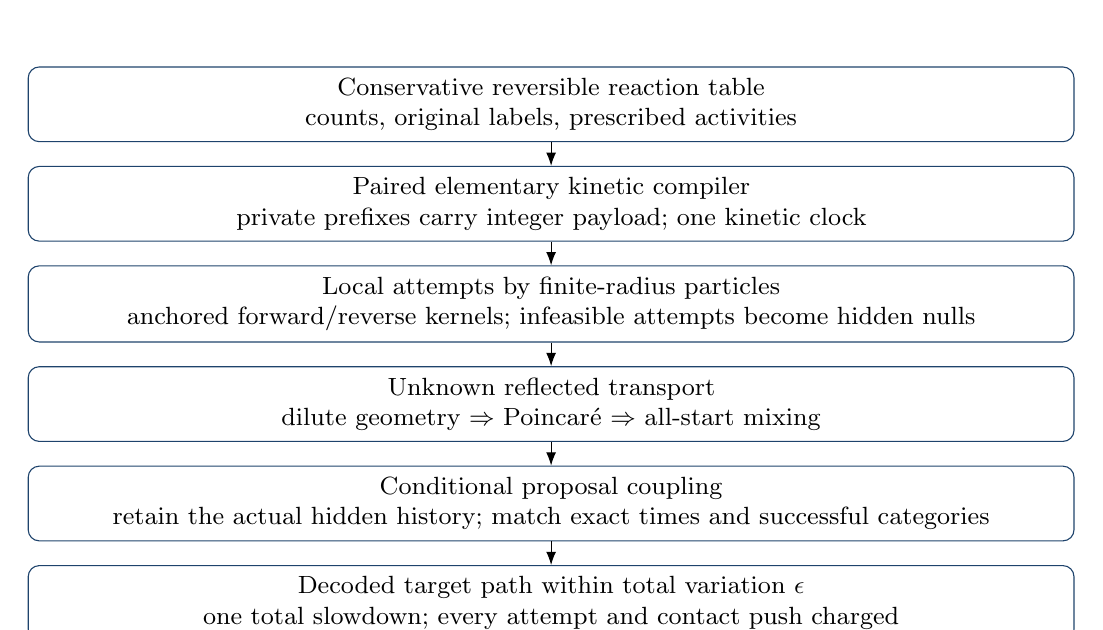
\begin{tikzpicture}[node distance=3mm,>=Latex,
 box/.style={draw=linkblue,rounded corners,align=center,text width=13cm,
 inner sep=4pt,font=\small}]
\node[box](a){Conservative reversible reaction table\\
counts, original labels, prescribed activities};
\node[box,below=of a](b){Paired elementary kinetic compiler\\
private prefixes carry integer payload; one kinetic clock};
\node[box,below=of b](c){Local attempts by finite-radius particles\\
anchored forward/reverse kernels; infeasible attempts become hidden nulls};
\node[box,below=of c](d){Unknown reflected transport\\
dilute geometry $\Rightarrow$ Poincar\'e $\Rightarrow$ all-start mixing};
\node[box,below=of d](e){Conditional proposal coupling\\
retain the actual hidden history; match exact times and successful categories};
\node[box,below=of e](f){Decoded target path within total variation $\epsilon$\\
one total slowdown; every attempt and contact push charged};
\draw[->](a)--(b);\draw[->](b)--(c);\draw[->](c)--(d);
\draw[->](d)--(e);\draw[->](e)--(f);
\end{tikzpicture}

% End figures/pipeline.tex

\caption{The compilation argument. Buffers, rank maps, metric projections
and random coordinate paths occur only in proofs. They are not forces or
relocation operations in the emitted system.}
\label{fig:pipeline}
\end{figure}

Three issues require care. First, exact balance is a local flux identity,
whereas accurate well-mixed kinetics is an averaging statement. The former
holds exactly for successful nominal jumps; the latter pays the small
excluded-volume bias. Second, small excluded volume does not by itself prove
mixing from a touching configuration. The hard-ball Poincar\'e proof and local
reflection estimates address that distinct problem. Third, a perturbation
policy may read every hidden event. Replacing the physical history by fresh
equilibrium positions would change the policy. Our comparison changes only
an auxiliary reference category, leaving the actual physical history intact.

The radius is chosen before the extra spatial slowdown. The radius pays
stationary bias per proposal; the slowdown pays relaxation between proposals.
Thus the proof never asks a radius chosen at the start to be small relative
to a later, radius-dependent horizon.

\begin{table}[htbp]
\centering\small
\begin{tabular}{@{}p{.18\textwidth}p{.73\textwidth}@{}}
\toprule
Symbol & Meaning\\\midrule
$x,X_t$ & target count and reference-time target process\\
$Z_s,Q_s$ & fine counts and positions at physical time $s$\\
$P,d_s$ & payload matrix and unweighted payload size $d_s=|P_s|_1$\\
$N,H$ & conserved mass cap and total physical slowdown\\
$\rho,r$ & particle-size scale and encounter/placement range\\
$A_0,A$ & prescribed nominal block covariance and actual joint covariance\\
$\mu_\K$ & uniform probability on one labelled feasible configuration space\\
$L_*,J$ & deterministic proposal majorant and expected proposal-budget bound\\
\bottomrule
\end{tabular}
\caption{Notation guide. Reference time is $t$; the corresponding physical
time is $Ht$.}
\end{table}
\clearpage

% End sections/01_introduction.tex


% Begin sections/02_model.tex
\section{Model and main theorem}
\label{sec:model}

\subsection{Target chemistry and numerical charge}

A finite labelled reaction table consists of $m$ channels
$r:y_r\to z_r$ on $d$ species, with $y_r,z_r\in\N^d$ and
rational $0<k_r\le1$. Complexes are given as expanded lists of molecules.
Set $q_r=|y_r|_1$ and
$D=\max(1,\max_r|y_r|_1,\max_r|z_r|_1)$. With the ordered-slot convention,
the target intensity is
\begin{equation}\label{eq:target}
 k_r(x)_{y_r},\qquad (x)_y=\prod_i x_i(x_i-1)\cdots(x_i-y_i+1).
\end{equation}
There is no factorial division when a reactant is repeated. Labels may be
parallel or null; a null label still records a firing time.
Empty sums and maxima throughout are zero, with the explicit minimum
$D\ge1$ retained.

The input includes a reverse involution $r\mapsto\bar r$, with
$y_{\bar r}=z_r$, $z_{\bar r}=y_r$. A fixed label of the involution is null.
It includes rational activities $a_i>0$ and positive integers $\omega_i$ such
that, for every label,
\begin{equation}\label{eq:targetbalance}
 k_ra^{y_r}=k_{\bar r}a^{z_r},\qquad
 \omega\cdot y_r=\omega\cdot z_r.
\end{equation}
The initial count $x_0\in\N^d$ is binary encoded and
$N=N_0=\omega\cdot x_0$. The target chain is nonexplosive because its
conserved count set is finite.

The remaining rational input is $\tau>0$, $0<\epsilon<1/8$,
$0<d_0\le1$, $\Lambda\ge1$, $0<r\le1/8$, and a full-dimensional convex
polytope $\Omega\subset[-1,1]^3$. It is specified by $F$ nonzero rational
facet inequalities, with redundant inequalities allowed, a rational point
$c$, and $0<\kappa\le1$ certifying $B_\kappa(c)\subset\Omega$.
We write its inequalities as $n_f\cdot x\le b_f$, where $n_f$ is the
outward unit normal. These normalized coefficients may be algebraic.

Define the following numerical quantities before making an efficiency claim:
\begin{align}
 B&=1+\left\lceil\frac{256(N+1)}\epsilon\right\rceil,
 &U&=1+B,\nonumber\\
 \Gamma&=2+m+\sum_rk_rU^{q_r},
 &\Xi&=2+\left(2+\sum_i(a_i+a_i^{-1})\right)^{2D+2},
 \label{eq:charges}\end{align}
and
\begin{align}
\Rnum={}&2+d+m+D+F+\sum_i\omega_i+N+\tau+\tau^{-1}
 +\epsilon^{-1}+d_0^{-1}+\Lambda+r^{-1}+\kappa^{-1}\nonumber\\
 &+\Gamma+\sum_rk_r^{-1}+\Xi.\label{eq:Rnum}
\end{align}
Let $L$ be the complete binary input length. A polynomial in $\Rnum$ can
be very large as a function of $L$. In particular, variable reaction order,
activities, time and initial population are paid numerically.

\subsection{Particles, reactions and faults}

A fine species $s$ carries a nonzero column $P_s\in\N^d$. Put
$d_s=|P_s|_1$ and give it radius $\rho_s=\rho d_s$ for one computed
rational $\rho>0$. Fine counts $Z$ decode to $PZ$. For a current labelled
particle list of length $n$, let $s(i)$ denote species and $r_i=\rho_{s(i)}$.
The feasible positions are
\begin{equation}\label{eq:configuration}
 \K=\{q:n_f\cdot q_i\le b_f-r_i,\quad
             |q_i-q_j|\ge r_i+r_j\}.
\end{equation}
Labelling is an analytical device, consistent with exchangeability within a
species. Actual mass-action counts use ordered distinct slots.

Let $V=\Vol(\Omega)$, $v=(2r)^3$ and
\begin{equation}\label{eq:kernel}
 K_r(z)=v^{-1}\ind_{[-r,r]^3}(z).
\end{equation}
There is no periodic identification. A binary-to-unary channel acts on an
ordered pair at $x,y$ with nominal attempt rate $c_eVK_r(y-x)$ and retains
the anchor $x$. Its reverse acts on a parent at $x$ with attempt rate
$c_{\bar e}$ and draws an independent offset $z\sim K_r$, placing children
at $x,x+z$. Unary channels retain the center; binary-to-binary channels
retain their designated slots. A global $0\to0$ label has its stated rate.
A jump succeeds precisely when its proposed new configuration is feasible.
An infeasible attempt is recorded as a hidden null. The structural list of
such branches is specified in \cref{sec:localjumps}; success and rejection
branches have independently perturbed intensities. Neither branch is removed
because it is unlikely at a particular count or placement.

For each species, the unknown nominal diffusivity is a deterministic real
symmetric matrix $D_s(t,x)$ satisfying
\begin{equation}\label{eq:Dassumptions}
 d_0I\le D_s(t,x)\le I.
\end{equation}
It is $C^3$ in space up to the boundary, its spatial derivatives of orders
$1,2,3$ have operator norm at most $\Lambda$, and $D_s$ and its spatial
derivatives through order two are Lipschitz in time with constant at most
$\Lambda$. These bounds hold for all physical times. Set
\[
 g_s=\operatorname{div}D_s,\qquad
 A_0(t,q)=\diag(D_{s(i)}(t,q_i)).
\]
The divergence drift $g_s$ is part of the model, rather than an imposed
control. Between chemical events the positions obey
\begin{align}
 dQ_i={}&(g_{s(i)}(t,Q_i)+v_i)\dt+[\sqrt{2A}\dd W]_i
 -\sum_fD_{s(i)}(t,Q_i)n_f\dd L_{if}\nonumber\\
 &+\sum_{j\ne i}D_{s(i)}(t,Q_i)e_{ij}\dd L_{ij},
 \qquad e_{ij}=\frac{Q_i-Q_j}{|Q_i-Q_j|}.\label{eq:SDE}
\end{align}
Each $L_{if}$ is continuous nondecreasing and grows only at the indicated
wall contact. The common $L_{ij}=L_{ji}$ grows only at pair contact.
They are reset as lifetime clocks when the particle list changes.

For a computed $0<\delta\le1/4$, allowed faults satisfy, predictably,
\begin{equation}\label{eq:faults}
 |v_i|\le\delta,\qquad A=A^\top,\quad
 \norm{A-A_0}_{\mathrm{op}}\le\delta d_0,
\end{equation}
and multiply every success, rejection and other chemical branch separately
by a factor in $[1-\delta,1+\delta]$. The joint matrix $A$ need not be block
diagonal. Faults may depend on the full continuous history, hidden and null
events, contact clocks and external randomness, but not on future innovations.
Reflection in \eqref{eq:SDE} remains the \emph{nominal block-conormal}
reflection; it is not replaced by conormal reflection for $A$.

An \emph{admitted realization} is a process satisfying these equations and
clock conditions with Brownian and reaction innovations relative to its
filtration. The theorem covers every such realization and every admitted
clock decomposition. We also prove existence and uniqueness of the nominal
position process, including from touching configurations. Existence for an
arbitrary pathological feedback specification is not an additional assertion.

\subsection{Path observation and theorem}

The retained record is the initial decoded count together with the ordered
list $(t_j,r_j,x_j)$ of original-labelled firings and post-firing decoded
counts. The exact real time coordinates are part of this measurable record.
Original null and parallel labels are kept. Positions, private reactions and
steric rejections are hidden. For laws $\nu,\nu'$ on this record space,
$\TV(\nu,\nu')=\sup_E|\nu(E)-\nu'(E)|$.

\begin{theorem}[Finite-radius spatial compilation]\label{thm:main}
There are computable universal constants $C,p$ and a deterministic compiler
with the following properties for every input in \cref{sec:model}.
It emits an elementary labelled network, payload matrix $P$ equal to the
identity on original species, positive rational activities $\widetilde a_s$
with $\widetilde a_i=a_i$, positive rational coefficients $c_e\le1$, one
positive rational radius scale $\rho$, a rational slowdown $H\ge1$ and a
rational tolerance $\delta>0$.

The species, base-channel and payload structure depends only on the reaction
list and reverse involution. Every column of $P$ is nonzero and
\begin{equation}\label{eq:radiusceiling}
 \rho(1+N+P_{\max})\le\frac{\min(\kappa,r)}{2^{16}},
 \qquad P_{\max}=\max_s|P_s|_1.
\end{equation}
Every actual reverse pair satisfies
$c_e\widetilde a^{\alpha_e}=c_{\bar e}\widetilde a^{\beta_e}$,
with the designated reverse labels. These are nominal algebraic identities.

For all finite fine counts $u,w$,
\begin{equation}\label{eq:graphmain}
 u\leadsto w\quad\Longleftrightarrow\quad Pu\leadsto Pw,
\end{equation}
and communicating classes are the corresponding preimages. On the physical
cap $\omega\cdot Pz\le N$, every count has strictly feasible configurations,
and every finite allowed count path has positive-probability spatial
realizations from every feasible initial placement.

Initialize exactly $x_0$ original particles at any feasible deterministic
positions and no auxiliaries. For every profile satisfying
\eqref{eq:Dassumptions} and every admitted fault realization,
\begin{equation}\label{eq:pathmain}
 \TV\bigl(\mathcal L(\text{observed physical path at times }Ht,
                      \,0\le t\le\tau),\mathcal L(X_{[0,\tau]})\bigr)
 \le\epsilon.
\end{equation}
No initial interval or internal waiting time is deleted.

The nominal diffusion and successful jumps have a common restricted Poisson
reference measure, as specified in \cref{prop:balance}. For all actual
physical times $s\ge0$, $|Z_s|_1\le N$ pathwise, the process is nonexplosive,
and all the resource bounds of \cref{thm:resources} hold. Compiler time,
memory, output length, $H,H\tau,\rho^{-1},\delta^{-1}$, positive coefficient
and activity inverses, and the stated horizon resource bounds are at most
\begin{equation}\label{eq:complexitymain}
 C(1+L+\Rnum)^p.
\end{equation}
The compiler does not query the unknown profiles or compute a
configuration-space normalizer, a PDE, a metric projection or a path-law
sampler.
\end{theorem}

The abstract graph assertion \eqref{eq:graphmain} concerns finite integer
counts without a packing interpretation. Its spatial assertion is restricted
to the conserved cap. In particular, the theorem does not claim that an
unbounded number of positive balls fits in a bounded vessel.

% End sections/02_model.tex


% Begin sections/03_chemistry.tex
\section{Elementary chemistry and exact spatial balance}
\label{sec:chemistry}

\subsection{The precise kinetic interface}

The first compiler operates on counts. We record its contract so that the
spatial proof has a public, noncircular dependency.

\begin{proposition}[Paired kinetic interface, {\cite[Theorem~9.1]{Sandhu2026}}]
\label{prop:kinetic}
For the chemical data of \cref{sec:model}, duration $\tau$ and accuracy
$\epsilon/8$, a deterministic algorithm produces $d+J_0$ species and
$2J_0+m$ channels, where $J_0=\sum_rq_r$, a nonzero-column integer payload
matrix $P$ with $P_{\max}\le D$, activities $\widetilde a_s$, normalized
coefficients $0<b_e\le1$, a clock $H_{\rm kin}\ge1$ and tolerance
$\delta_{\rm kin}>0$. Base channels are $2\leftrightarrow1$, unary-to-unary,
and global $0\to0$ channels. They have the graph and label properties in
\cref{thm:main}, conserve $\omega\cdot PZ$, and are exactly detailed balanced
at $\widetilde a$. From $(x_0,0)$ their complete decoded marked path on
$[0,H_{\rm kin}\tau]$, rescaled by $H_{\rm kin}$, is within $\epsilon/8$
of the target, under every full-history predictable relative chemical fault
of size at most $\delta_{\rm kin}$.

With $W_b$ as in that theorem, $W_b\le8\Rnum$. Every numerical output,
including $H_{\rm kin}$, $H_{\rm kin}\tau$, $\delta_{\rm kin}^{-1}$,
$\max_eb_e^{-1}$ and $\max_s(\widetilde a_s+\widetilde a_s^{-1})$,
is bounded by $2^{1024}W_b^{128}$. Its bit work, memory and output length
are at most $2^{1024}(1+L)^{128}$.
\end{proposition}

The cutoff used by the cited theorem is
$1+\lceil32(N+1)/(\epsilon/8)\rceil$, exactly $B$ in
\eqref{eq:charges}. Thus its variable-order activity charge and $\Gamma$
are the same quantities, rather than estimates at an uncharged larger
cutoff. All its other hypotheses are precisely \eqref{eq:targetbalance}.
The theorem is proved independently of any spatial construction.

For orientation, its paired construction can be described explicitly.
For every directed source list $y_r=(i_1,\ldots,i_{q_r})$, make private
prefixes $S_{r,j}$ of payload $\sum_{h\le j}e_{i_h}$, $2\le j\le q_r$,
and a pending species $C_r$ of payload $y_r$ when $q_r>0$. The chains are
\[
 X_{i_1}+X_{i_2}\rightleftarrows S_{r,2},\quad
 S_{r,j-1}+X_{i_j}\rightleftarrows S_{r,j},\quad
 S_{r,q_r}\rightleftarrows C_r.
\]
For a unary source the chain is $X_{i_1}\rightleftarrows C_r$; an empty
conservative source has an empty product and uses a global null channel.
Central observed channels are $C_r\to C_{\bar r}$ with label $r$.
Release to originals connects every fibre to its canonical state.
Hence every fine transition decodes correctly, and every target edge lifts;
this proves the exact graph assertion without count enumeration.

To see why the paired lift is balanced, assign relative weights
$w(S_{r,j})=\vartheta U^{-j}$ and
$w(C_r)=\vartheta U^{-q_r}$, and absolute activities
$\widetilde a_s=w(s)a^{P_s}$, with original relative weight one.
First binding/release coefficients before normalization are
$K\vartheta/U^2,K$; subsequent ones are $K/U,K$; full-prefix/pending
coefficients are $K,K$; unary entry/return coefficients are
$K\vartheta/U,K$. A central coefficient is
$Qk_rU^{q_r}$. Each central balance identity reduces to
$Q\vartheta k_ra^{y_r}=Q\vartheta k_{\bar r}a^{z_r}$.
The quantitative fast-fibre and marked-filter argument determining
$\vartheta,K,Q$ and the common normalization is the proof of the cited
theorem. In particular, it includes every post-event layer and original
null mark. Reversibility is obtained by this paired construction, rather
than by restricting an irreversible compiler to a conservative table.

\subsection{Local jumps and structural rejection}
\label{sec:localjumps}

For a base channel, use the placement rule of \cref{sec:model}. Add one
hidden rejection branch precisely in the following cases:
\begin{center}\small
\begin{tabular}{@{}ll@{}}\toprule
Base type & Condition for a rejection branch\\\midrule
$1\to2$ & Always\\
$1\to1$ & The retained slot grows\\
$2\to2$ & At least one retained slot grows\\
$2\to1$ & The anchored product grows beyond the anchored reactant\\
\bottomrule\end{tabular}
\end{center}
The branch retains all reactant slots and their species, and fires only on
the failure set of its base placement. Thus a binary rejection is a binary
null channel with the \emph{inherited failure kernel}, not an unrestricted
identity-placement channel. The base network in \cref{prop:kinetic} needs
binary-to-binary channels only for these null branches.

If no retained slot grows and no new slot is added, feasibility is preserved
by removal and shrinking, proving that no rejection branch is possible.
A $1\to2$ release fails for sufficiently small offsets. A growing slot can
be placed near a supporting face so that its larger replacement fails.
The other particles can be parked in the inball. These are open sets of
placements and, where needed, offsets. A supporting face nearest $c$ gives
a usable patch without a lower bound on an individual facet's area. Tiny
radii relative to $\kappa$ leave the patch and parking region separated.
Consequently the rejection list is structural and independent of population
or numerical geometry. A genuine identity null has identical slot radii and
always succeeds, retaining its original label.

At zero faults, the success and failure coefficients are the same. Under
faults their multipliers are independent. For example, if $w(q)$ is a
release-success probability at the current placement, its actual combined
attempt rate is
\[
 c\{\alpha_{\rm suc}w(q)+\alpha_{\rm rej}(1-w(q))\}.
\]
This need not be constant. The proof below uses a majorizing proposal
process, rather than treating this rate as an unperturbed Poisson clock.

\subsection{The encounter normalizer}

The point-particle normalization is the rational number
\begin{equation}\label{eq:q}
 q=\frac1V\int_{\Omega^2}K_r(y-x)\dd x\dd y,
 \qquad \frac{\kappa^6}{4096}\le q\le1.
\end{equation}
The upper bound follows by integrating the probability kernel. For the
lower bound, put $s=\min(\kappa/2,r)$ and integrate over
$x\in B_{\kappa/2}(c)$, $z\in B_s(0)$, $y=x+z$. These pairs lie in
$\Omega^2$ and in the cube kernel. Their contribution is at least
$\pi^2\kappa^3\min(\kappa/(2r),1)^3/288$. Using $r\le1/8$ and
$\kappa\le1$ gives the displayed conservative lower bound.
The double integral is a six-dimensional rational polytope volume divided
by $Vv$. Its exact finite-bit calculation is given in
\cref{app:arithmetic}. No hard-ball configuration volume is calculated.

After an extra integer slowdown $h$, set
\begin{equation}\label{eq:spatialrates}
 c_e=\begin{cases}b_e/(hq),&e\text{ belongs to a binding/release pair},\\
                  b_e/h,&e\text{ is unary or global null}.
       \end{cases}
\end{equation}
Rejection branches inherit the corresponding base coefficient. Reverse
pairs receive the same factor, preserving all activity identities exactly.

\begin{proposition}[Exact nominal flux]\label{prop:balance}
At zero faults the successful spatial jump kernels satisfy detailed balance
with the Poisson point measure of intensities $\widetilde a_s/V$, restricted
to feasible configurations and to any invariant chemical class or conserved
cap. The fixed-count nominal diffusion has the instantaneous symmetric form
\begin{equation}\label{eq:form}
 \cE_t(f,g)=\int_\K\nabla f^\top A_0(t,q)\nabla g\dd\mu_\K,
 \qquad \operatorname{Dom}\cE_t=H^1(\K).
\end{equation}
Uniform measure $\mu_\K$ is common to these forms. A restricted measure is
normalized only when it has positive mass; every count beneath our cap
has strictly feasible configurations. These assertions do not state
reversibility of a time-ordered evolution or of a faulted marginal.
\end{proposition}
\begin{proof}
Fix the untouched configuration $\eta$ and a reversible binding
$A+B\rightleftarrows C$. The two successful Palm fluxes have the same
geometric measure
\[
 K_r(y-x)\ind_{\K}(\eta+A_x+B_y)
             \ind_{\K}(\eta+C_x)\dd x\dd y.
\]
Their scalar factors are, respectively,
\[
 \frac{c_e\widetilde a_A\widetilde a_B}{V}
 \quad\text{and}\quad\frac{c_{\bar e}\widetilde a_C}{V}.
\]
These are equal. Ordered identical-reactant slots give the factorial Palm
factor $\widetilde a_A^2$, with no division by two. This also follows directly
by cancellation of the count factorial with the falling factorial.
Unary retained-center fluxes have the same feasible source/target indicator
and equal activity factors. Rejections and global nulls are diagonal
configuration fluxes. Restricting both endpoints to an invariant set
preserves each equality. No normalizer enters this calculation.

The nominal generator is
$\operatorname{div}(A_0\nabla)$ because the intrinsic drift is
$\operatorname{div}A_0$. Integration by parts gives \eqref{eq:form} with
conormal Neumann boundary. The construction from all boundary starting
points and the identification of this form are proved in
\cref{app:existence}. In particular, constants are preserved and the
uniform measure is invariant at every time.
\end{proof}

For a fine count $z$, the reference count weight is proportional to
\begin{equation}\label{eq:countweight}
 \frac{\widetilde a^z}{z!}\,
 \frac{\Vol(\K_z)}{V^{|z|_1}}.
\end{equation}
The excluded-volume factor depends on $z$. In addition the kinetic decoder
has its own fibre partition correction. Neither correction is suppressed;
the decoded equilibrium is not asserted to be the target's unconditional
Poisson count law.

\begin{example}[A boundary rejection in $2A\rightleftarrows B$]
\label{ex:binary}
Take both target rates and activities equal to one and weights
$\omega_A=1$, $\omega_B=2$. The forward prefix and pending species carry
$2A$; the reverse pending species carries $B$. Their radii are
$2\rho,2\rho,\rho$, respectively: radii use unweighted payload size,
not conserved mass. An elementary binding $A+A\to S$ anchors the product
of radius $2\rho$ at the first center. It may fail near a wall even when
the two reactants fit. Its reverse samples the offset in the same cube and
checks both offspring. The two successful fluxes contain exactly the same
pair of feasibility indicators, so rejecting one orientation without the
corresponding indicator in the other would break balance. The failure is a
hidden attempt; it is not an observed $2A\to B$ event.

For the unit cube $[-1/2,1/2]^3$, the point-particle normalizer is explicitly
$q=(1-r/2)^3$. It is neither the release-success probability at every parent
position nor the hard-ball count normalizer in \eqref{eq:countweight}.
\end{example}

% End sections/03_chemistry.tex


% Begin sections/04_geometry.tex
\section{Dilute hard-ball geometry}
\label{sec:geometry}

All fixed-count arguments use only
$n\le N$, $r_i=\rho d_i$, $d_i\ge1$ and $\sum_i d_i\le N$.
Write the inward gaps
\begin{equation}\label{eq:gaps}
 g_{if}=b_f-n_f\cdot q_i-r_i,\qquad
 g_{ij}=|q_i-q_j|-r_i-r_j,
\end{equation}
whose gradients have norms one and $\sqrt2$. There are at most
$J_c=nF+n(n-1)/2$ constraints. The empty configuration requires no estimates.

\subsection{A common inward direction}

\begin{lemma}[Contact cone]\label{lem:cone}
Under $\rho(1+N)\le\kappa/2^{16}$, at every feasible configuration there
is a unit vector $v$ with
\begin{equation}\label{eq:alpha}
 \nabla g_j\cdot v\ge\alpha,
 \qquad \alpha=\frac{\kappa}{2^{10}(1+N)^2},
 \qquad g_j\le\rho.
\end{equation}
For every nonnegative combination of active conormals,
\begin{equation}\label{eq:nocirculation}
 \left|\sum_j\lambda_jA_0\nabla g_j\right|
       \ge d_0\alpha\sum_j\lambda_j.
\end{equation}
\end{lemma}
\begin{proof}
Join particles when their pair gap is at most $\rho$. In each connected
cluster $C$, put $R_C=\sum_{i\in C}r_i$ and let $z_C$ be the arithmetic
mean of its centers. Along a simple connecting path, each edge has length
at most $r_i+r_j+\rho$; thus the cluster diameter is at most $3R_C$.
Use the unnormalized direction
\[
 v_i=\frac{16R_C}{\kappa}(c-z_C)+(q_i-z_C),\qquad i\in C.
\]
For a near pair its gap derivative is $|q_i-q_j|\ge2\rho$.
For a near wall,
$n_f\cdot(c-z_C)\le-\kappa+5R_C\le-\kappa/2$,
so $n_f\cdot v_i\le-8R_C+3R_C\le-5\rho$.
Finally $|v|\le60\rho N^{3/2}/\kappa$. Normalization gives
\eqref{eq:alpha} with room to spare. Pairing the conormal sum with
$A_0^{-1}v$, whose norm is at most $d_0^{-1}$, gives
\eqref{eq:nocirculation}.
\end{proof}

The angle $\alpha$ is independent of $\rho$. The neighborhood on which it
works shrinks with $\rho$, which will determine a short time scale. In
particular a positive circulation of contact clocks cannot hide a large
unsigned push behind a zero resultant.

\subsection{Poincar\'e by buffering, separation and coordinate paths}

\begin{theorem}[Dilute hard-ball Poincar\'e inequality]\label{thm:poincare}
Let $\rho=a^2$ for a positive rational $a$ satisfying
\begin{equation}\label{eq:atiny}
 a\le2^{-30}(2+N+F+\kappa^{-1})^{-20}.
\end{equation}
For every count beneath the cap and every $f\in H^1(\K)$,
\begin{equation}\label{eq:CP}
 \Var_{\mu_\K}f\le C_P\int_\K|\nabla f|^2\dd\mu_\K,
 \qquad C_P=2^{20}(1+N).
\end{equation}
\end{theorem}

The obstacle to a direct product comparison is geometric. A line joining
two feasible configurations can cross a collision surface; freezing all but
one particle can even create a cage. We first move each endpoint a little,
with controlled density distortion. The moved endpoints are well separated.
A randomly chosen intermediate configuration then supplies two admissible
one-particle-at-a-time paths with uniformly positive probability.

\begin{proof}
We prove the inequality for smooth functions, then extend it.

\emph{Step 1: create a tiny buffer.}
Choose $0\le\chi\le1$, equal to one on $(-\infty,1/4]$, zero on
$[1/2,\infty)$ and Lipschitz with constant eight. Extend pair gradients
by replacing $(q_i-q_j)/|q_i-q_j|$ with
$(q_i-q_j)/\max(|q_i-q_j|,\rho)$; denote the constraint vectors by $b_j$.
They equal $\nabla g_j$ on $\K$. Let $V(q)$ minimize
\begin{equation}\label{eq:Vmin}
 \frac12|v|^2+8\alpha^{-2}\sum_j
 \chi(g_j(q)/\rho)[1-b_j(q)\cdot v]_+^2,
\end{equation}
and clip it to $|v|\le\alpha^{-1}$. On $\K$ the direction in
\cref{lem:cone}, divided by $\alpha$, makes every active penalty zero.
Comparison with it proves that clipping has no effect and $|V|\le\alpha^{-1}$.
For $g_j\le\rho/4$, comparison of that one penalty gives
$\nabla g_j\cdot V\ge3/4$.

Strong convexity of \eqref{eq:Vmin} gives the global safe estimate
\begin{equation}\label{eq:VLip}
 \Lip(V)\le L_V=\frac{2^{16}(1+J_c)^2}{\alpha^3\rho}.
\end{equation}
For completeness, comparison with $v=0$ first bounds the untruncated
minimizer by $4\sqrt{J_c}/\alpha$. Subtract the two minimizer equations,
pair with their difference, and use strong monotonicity on the left.
The coefficient differences on the right are bounded using
$\Lip(b_j)\le4/\rho$, $\Lip(\chi\circ(g_j/\rho))\le16/\rho$
and this minimizer bound. Their sum is at most the right side of
\eqref{eq:VLip} times the displacement. Radial clipping is nonexpansive.

Set
\begin{equation}\label{eq:buffereta}
 \eta=64\rho^3(1+N)^5\kappa^{-2},
\end{equation}
and let $B_s$ be the flow of $V$ for time $2\eta s$, $0\le s\le1$.
The positive derivative of every small gap proves forward invariance and
$B_1\K\subset\K_\eta:=\{g_j\ge\eta\}$. The flow is injective, with
inverse Lipschitz constant $e^{2\eta L_V}$. Hence its volume distortion is
at most $e^{6n\eta L_V}$. If $G_0=2+N+F+\kappa^{-1}$, then
\[
 6n\eta L_V\le2^{55}\rho^2G_0^{21}<\log2
\]
by \eqref{eq:atiny}. Thus $(B_s)_\#\mu_\K\le2\mu_\K$, and integration
along the flow gives
\begin{equation}\label{eq:bufferenergy}
 \int|f-f\circ B_1|^2\dd\mu_\K
 \le8\eta^2\alpha^{-2}\int|\nabla f|^2\dd\mu_\K.
\end{equation}

\emph{Step 2: separate by rank without a factorial penalty.}
For buffered $x$, sort the first coordinates and put
$k_i=\operatorname{rank}(x_{i1})-(n+1)/2$, breaking ties by label. Define
\begin{equation}\label{eq:rankmap}
 \theta=4an/\kappa,\qquad
 S_s(x)_i=(1-s\theta)x_i+s\theta c+sa k_i e_1.
\end{equation}
For a wall, its gap is at least
$(1-s\theta)\eta+s\theta(\kappa-r_i)-sa|k_i|\ge\eta$.
For a pair, put $z=x_i-x_j$, $k=k_i-k_j$. Sorting gives $z_1k\ge0$
and $|k|\ge1$, so
\begin{align}
 |S_s(x)_i-S_s(x)_j|^2
 &\ge(1-s\theta)^2|z|^2+s^2a^2k^2\nonumber\\
 &\ge\frac{|z|^2}{1+\theta^2|z|^2/(a^2k^2)}.\label{eq:rankpair}
\end{align}
The last bound is obtained by minimizing the quadratic over all real $s$.
It increases with $|z|^2$. With $R=r_i+r_j\le\rho N$ and
$|z|\ge R+\eta$, its possible loss in length is at most
$8n^2(R+\eta)^3/\kappa^2$. Condition \eqref{eq:atiny} gives
$\eta\le\rho N/8$ when $N\ge1$, and the loss is less than $\eta/4$
by \eqref{eq:buffereta}. Thus the whole path is strictly pair feasible.
Its endpoint has first-coordinate separations at least $a$.

On each rank chamber the Jacobian is $(1-s\theta)^{3n}\ge1/2$.
The output ordering recovers the input chamber. Distinct chamber images
are disjoint: summing their density contributions costs no factor $n!$.
Tie sets and their preimages under the bi-Lipschitz buffer have measure
zero. The squared speed is at most
$A_{\rm rank}^2=2^{10}\rho n^3\kappa^{-2}$.
For $T=S_1B_1$ and $\lambda=T_\#\mu_\K$, we have
\begin{align}
 \lambda&\le4\mu_\K,\label{eq:lambdadensity}\\
 \int|f-f\circ T|^2\dd\mu_\K
 &\le(16\eta^2\alpha^{-2}+8A_{\rm rank}^2)
                      \int|\nabla f|^2\dd\mu_\K.\label{eq:rankenergy}
\end{align}

\emph{Step 3: compare through a common intermediate point.}
Let $\Omega_i=\{x:n_f\cdot x\le b_f-r_i\}$ and
$\nu=\bigotimes_i\Unif(\Omega_i)$. Then $\mu_\K=\nu(\cdot\mid\K)$.
Each $\Omega_i$ contains $B_{\kappa/2}(c)$. A union bound for pair
exclusion, using the volume of a three-dimensional ball, gives
$\nu(\K)\ge1/2$ under \eqref{eq:atiny}.

Starting at an $a$-separated configuration $u$, draw $z\sim\nu$ and move
particle $1$ from $u_1$ to $z_1$, then particle $2$, and so on. Walls remain
feasible by convexity. For an unmoved obstacle $u_j$, $j>i$, endpoints
$z_i$ producing a collision with its exclusion ball occupy a solid-angle
cone of probability at most
$C(r_i+r_j)^2/(\kappa^3a^2)$: the cone angle is at most a constant times
$(r_i+r_j)/|u_i-u_j|$, and its length is bounded by the vessel diameter.
For a moved obstacle $z_j$, condition on $z_i$. Its bad locations occupy
a tube about $[u_i,z_i]$, of probability at most
$C(r_i+r_j)^2/\kappa^3$.
Because
\[
 \sum_{i<j}(d_i+d_j)^2
 =(n-2)\sum_i d_i^2+\Big(\sum_i d_i\Big)^2\le N^3,
\]
the probability that the entire path fails is at most
\begin{equation}\label{eq:badpath}
 \beta=2^9\kappa^{-3}\rho^2N^3(1+a^{-2})\le\tfrac14.
\end{equation}
For any two separated endpoints $u,w$, a common $z$ supports both paths
with probability at least $1-2\beta\ge1/2$.

To bound their energies, during segment $i$ the current configuration is
\[
 (z_1,\ldots,z_{i-1},(1-s)u_i+sz_i,u_{i+1},\ldots,u_n).
\]
For $s\le1/2$ change variables from $u_i$ to the current coordinate; for
$s\ge1/2$ change from $z_i$. Each Jacobian is at most $2^3=8$.
All other unused coordinates integrate out. Using
$\lambda\le4\nu/\nu(\K)$ and retaining the valid-path indicator, the
remaining energy integral is over $\K$; its factor $\nu(\K)$ cancels.
Segment lengths squared are at most $12$. Cauchy--Schwarz over the $n$
segments gives integrated energy at most $384n\int|\nabla f|^2\dd\mu_\K$
for one endpoint. The two paths, the inequality $|a+b|^2\le2a^2+2b^2$,
and the validity normalization at most two yield
\begin{equation}\label{eq:Varlambda}
 \Var_\lambda f\le1536n\int|\nabla f|^2\dd\mu_\K.
\end{equation}
Only one three-dimensional coordinate was interpolated at a time.

Choose the mean of $f$ under $\lambda$ as a comparison constant and use
\eqref{eq:rankenergy} and \eqref{eq:Varlambda}. We obtain
\[
 \Var_{\mu_\K}f\le
 (32\eta^2\alpha^{-2}+16A_{\rm rank}^2+3072n)
                         \int|\nabla f|^2\dd\mu_\K.
\]
Condition \eqref{eq:atiny} absorbs the first two terms into
$2^{20}(1+N)$. Finally, the cone condition makes $\K$ a bounded Lipschitz
domain. Sobolev extension and smooth density extend the inequality to
$H^1(\K)$. No quantitative extension constant enters the proved estimate.
\end{proof}

\begin{figure}[htbp]\centering

% Begin figures/coordinate_paths.tex
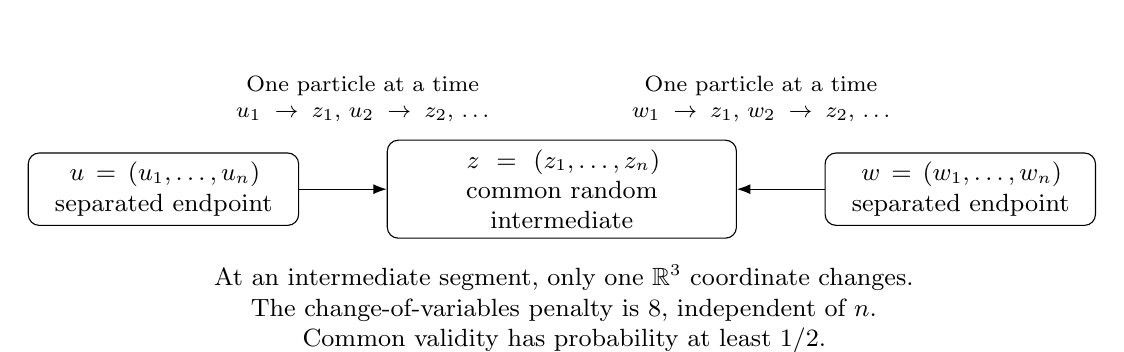
\begin{tikzpicture}[>=Latex,scale=.92,every node/.style={font=\small}]
\node[draw,rounded corners,align=center,text width=3.2cm](u) at (0,0)
 {$u=(u_1,\ldots,u_n)$\\separated endpoint};
\node[draw,rounded corners,align=center,text width=4.2cm](z) at (5.5,0)
 {$z=(z_1,\ldots,z_n)$\\common random\\intermediate};
\node[draw,rounded corners,align=center,text width=3.2cm](w) at (11,0)
 {$w=(w_1,\ldots,w_n)$\\separated endpoint};
\draw[->](u)--(z);
\draw[<-](z)--(w);
\node[align=center,text width=4.5cm,font=\footnotesize] at (2.75,1.25)
 {One particle at a time\\$u_1\to z_1$, $u_2\to z_2$, $\ldots$};
\node[align=center,text width=4.5cm,font=\footnotesize] at (8.25,1.25)
 {One particle at a time\\$w_1\to z_1$, $w_2\to z_2$, $\ldots$};
\node[align=center,text width=13cm] at (5.5,-1.65)
 {At an intermediate segment, only one $\R^3$ coordinate changes.\\
The change-of-variables penalty is $8$, independent of $n$.\\
Common validity has probability at least $1/2$.};
\end{tikzpicture}

% End figures/coordinate_paths.tex

\caption{The path comparison in \cref{thm:poincare}. The endpoint rank
deformation also has disjoint chamber images, avoiding a separate $n!$
density loss. These are integration paths, not particle controls.}
\label{fig:coordinates}
\end{figure}

\subsection{Feasibility and support}

The preceding construction proves more than an integral inequality. Every
feasible point can be buffered and rank-separated by a continuous feasible
path, strictly feasible after the initial buffer. Any two separated points
share valid intermediate points of positive volume. Almost every such
intermediate avoids tangencies, giving strictly feasible coordinate segments.
Thus every feasible starting configuration connects to any prescribed
interior neighborhood. Strict configurations also exist directly by putting
the capped particles in separated slots along a line in $B_\kappa(c)$.

Uniform ellipticity and a bounded-drift Girsanov guide along a finite
piecewise smooth interior path give positive probability of following a
small tube. At an initial contact, use the inward buffer and the short
reflection estimate in \cref{lem:localservices}; then use interior segments.
Equivalently the metric error estimate in \cref{app:comparison}, with the
guide drift, gives positive endpoint probability on sufficiently short
segments. Here are the quantitative facts needed for this qualitative
use. Subdivide the guide until each segment has displacement small relative
to the local cone radius. Traverse one segment in time $u$ with its
prescribed guide drift. The core argument bounds the conditional expected
clock by $C\sqrt u$ plus a polynomial constant times that segment's
length. Further subdivision makes the latter small enough for an
exponential clock bound. Applying the metric comparison to the actual
motion and the deterministic feasible guide then gives mean squared
endpoint error at most $C'u$. Choose $u$ smaller than a fixed fraction of
the squared clearance of the desired endpoint neighborhood. Markov's
inequality gives positive probability of entering it. The guide has finite
bounded speed on each chosen segment. Uniform ellipticity makes its
Girsanov density strictly positive with finite finite-horizon exponential
bound. Thus the same event has positive probability under the original
drift. This argument applies to the initial inward segment as well as
strict interior segments. This qualitative argument
is valid under adapted covariance faults as well: its inverse covariance is
uniformly bounded, and no derivative of the fault is used.
An independent proposal-free gap has positive probability. At suitable
interior placements every enabled successful channel has positive intensity
and a positive-volume set of successful offsets. The failure placements in
\cref{sec:localjumps} give the same conclusion for each listed rejection.
Iteration proves finite-path support. No polynomial lower bound on these
individual path probabilities is claimed or used in the accuracy estimate.

% End sections/04_geometry.tex


% Begin sections/05_transport.tex
\section{Unknown transport and conditional mixing}
\label{sec:transport}

The nominal reference measure is known as a mathematical object: it is
uniform on $\K$. Its normalizing volume is not known to the compiler.
Unknown diffusivity affects the rate of relaxation, but not this measure.
To exploit this fact we need estimates uniform over counts, initial contacts,
time origins and permitted coefficient profiles.

We give an intentionally coarse explicit ledger. Define
\begin{equation}\label{eq:master}
 Z_*=2+N+F+\kappa^{-1}+\rho^{-1}+d_0^{-1}+\Lambda+r^{-1},
 \qquad \mathsf M=2^{1024}Z_*^{1024}.
\end{equation}
The large fixed powers organize resource dependencies; they are not proposed
performance estimates. Set
\begin{equation}\label{eq:services}
 \ell=\mathsf M^{-16},\quad G=\mathsf M^{12},\quad
 b(g)=\min\{2,\mathsf M^{16}e^{-g/\mathsf M^4}\},\quad
 I=\mathsf M^6,\quad W=\mathsf M^{64}.
\end{equation}
Only $I,W$ are evaluated for the final parameter choices. The exponential
envelope is a proof device; no transcendental number is output.

\begin{lemma}[Local reflected services]\label{lem:localservices}
For every fixed capped count, the nominal equation has a unique position
process from every $q\in\K$, with form \eqref{eq:form}. Its evolution is
denoted $P^0_{s,t}$. Let $\mathcal L$ be the sum of all wall clocks and
unordered pair clocks on a chemical-free interval.
Uniformly over full past histories and all admitted realizations:
\begin{enumerate}[label=(\roman*)]
\item For $0<u\le\ell$, $\E[\Delta\mathcal L\mid\mathcal F_s]
\le\mathsf M\sqrt u$. On such windows,
$\E[e^{8\mathsf M\Delta\mathcal L}\mid\mathcal F_s]\le2$.
\item Couple the actual and nominal motion from the same point with the
same Brownian innovation. For $u\le\ell$,
$\E[|Q_{s+u}-Q^0_{s+u}|\mid\mathcal F_s]\le\mathsf M^4\delta$.
\item For $u\in[\ell/2,\ell]$ and bounded measurable $f$,
$P^0_{s,s+u}f$ is Euclidean Lipschitz on $\K$ with constant at most
$G\norm f_\infty$. The same bound holds for the gradient norm and
boundary values.
\end{enumerate}
These constants do not depend on derivatives of the actual faults.
\end{lemma}

The proof occupies \cref{app:reflection}. Its main device is the distance
to a slightly tightened configuration core, measured in the nominal inverse
covariance metric. Each individual contact lowers this potential. This pays
unsigned clocks even at corners, then supplies the exponential moments
needed for comparison and smooth-boundary approximation. The smoothing
import is applied only on smooth approximants, with polynomial curvature
and local-time constants checked uniformly before taking the corner limit.

\begin{lemma}[Uniform nonautonomous mixing]\label{lem:mixing}
For all $s,g\ge0$ and $\norm f_\infty\le1$,
\begin{equation}\label{eq:mixing}
 \sup_{q\in\K}|P^0_{s,s+g}f(q)-\mu_\K f|\le b(g),
 \qquad \int_0^\infty b(g)\dd g\le I.
\end{equation}
\end{lemma}
\begin{proof}
Constants are preserved and all instantaneous forms have the same invariant
measure. Their energy identity and \cref{thm:poincare} give
\begin{equation}\label{eq:L2}
 \norm{P^0_{s,s+g}f-\mu_\K f}_2
 \le e^{-d_0g/C_P}\norm{f-\mu_\K f}_2.
\end{equation}
One may see this by reversing the time coordinate in the backward equation
and differentiating the squared norm. No commutation or self-adjointness of
the full evolution is required.

Let $m_*=3n$. The contact cone and the pair Hessian bound give, on a radius
at least $\mathsf M^{-1}$,
\begin{equation}\label{eq:smallball}
 \mu_\K(B(q,u)\cap\K)
 \ge\left(\frac{\alpha u}{2^{12}\sqrt{m_*}}\right)^{m_*}.
\end{equation}
Indeed move a distance $u/2$ in a common inward direction and put a ball
of radius $\alpha u/16$ about that point. For sufficiently small $u$ the
quadratic gap loss is smaller than its linear gain; initially far
constraints remain far. The volume of an $m_*$-ball is at least
$(c/\sqrt{m_*})^{m_*}$, while $\Vol(\K)\le8^n$. The local geometric
constants are dominated by \eqref{eq:master}.

For $g\ge\ell$, smoothing the first short interval bounds the local
Lipschitz constant by $G$. If the centered function has maximum absolute
value $M_f$, it stays above $M_f/2$ in absolute value in a feasible ball
of radius $M_f/(2G)$. This radius is within the range of
\eqref{eq:smallball}. Consequently
\[
 M_f^{m_*+2}\le
 4\left(\frac{2^{13}G\sqrt{m_*}}\alpha\right)^{m_*}
 \norm{P^0_{s,s+g}f-\mu_\K f}_2^2.
\]
Taking the $(m_*+2)$th root makes the prefactor polynomial. By
\eqref{eq:master}, $m_*+2$, $C_P$ and $d_0^{-1}$ are each bounded by
$\mathsf M$; the resulting bound is at most
$\mathsf M^{16}e^{-g/\mathsf M^4}$. Short times are covered by two.
Integration gives at most
$\mathsf M^4(2+32\log\mathsf M)\le\mathsf M^6$.
For $n=0$ the centered function is zero.
\end{proof}

The small-ball volume has a dimension-dependent power. It is used only
before taking a dimension-dependent root; it never becomes a numerical
charge raised to the population. In particular we do not use a
high-dimensional pointwise heat-density bound.

\subsection{Conditional channel observables}

A normalized channel observable is the success or failure predicate of a
specified local placement, with its cube-contact factor, scaled to lie in
$[0,1]$. For release, integrate the predicate over the independent offset.
The only discontinuities are cube faces, shifted walls and pair-distance
surfaces involving an affected slot. For every such $f$ and $0<w\le1/2$
there are upper and lower functions satisfying
\begin{equation}\label{eq:sandwich}
 0\le f_w^-\le f\le f_w^+\le1,\quad
 \Lip(f_w^\pm)\le\mathsf M/w,\quad
 \mu_\K(f_w^+-f_w^-)\le\mathsf M w.
\end{equation}
For products of predicates, replace each step by a linear ramp of width
$w$ and bound the product difference by the sum of the individual ramp
differences. Pair distances and wall distances are uniformly Lipschitz.
The number of affected constraints is polynomial in $N+F$.
Each tube volume is three-dimensional: wall and cube slabs have volume
$O(w)$, and a distance-shell about a ball has volume
$O(w(R+w)^2)$. Current feasible-uniform measure is dominated by twice
product-uniform measure under \eqref{eq:atiny}; a release adds the density
factor $v^{-1}$. These observations prove \eqref{eq:sandwich}, including
its stated constants, as detailed in \cref{app:tubes}.

\begin{proposition}[Conditional occupation]\label{prop:occupation}
On a chemical-free gap of length $g$, starting at any feasible configuration,
every normalized channel observable satisfies
\begin{equation}\label{eq:occupation}
 \left|\E[f(Q_{s+g})\mid\text{full past}]-\mu_\K f\right|
       \le b(g)+W\delta^{2/9}.
\end{equation}
The same statement holds conditioned on the next independent proposal gap.
The motion during the gap may depend on its entire history.
\end{proposition}
\begin{proof}
For $g<2\ell$ the trivial bound is covered by $b(g)=2$. Otherwise split
the interval into subintervals of length in $[\ell/2,\ell]$ and telescope
the actual conditional transitions against the nominal future functions.
For a terminal ramp $f_w^\pm$, all but the last term have gradient at most
$G b(u)$, where $u$ is the remaining time after an initial smoothing
subinterval. By \cref{lem:localservices}(ii), their sum is at most
\[
 \mathsf M^4G\delta(4+4I/\ell)\le\mathsf M^{36}\delta.
\]
The last term is at most $\mathsf M^5\delta/w$.
Nominal mixing contributes $b(g)$ and the stationary sandwich contributes
$\mathsf M w$. This is conditional telescoping, so it assumes neither a
Markov fault policy nor independence between actual particles. Taking
$w=\sqrt\delta$ gives a bound at most
$b(g)+\mathsf M^{40}\sqrt\delta$, which is bounded by
\eqref{eq:occupation}. Larger ramp widths can be covered by the trivial
bound; here $\delta\le1/4$. Conditioning on the next independent proposal
gap leaves Brownian innovations and these conditional estimates unchanged.
\end{proof}

Thus robustness is proved through local comparisons and a summable
nominal future, rather than a synchronous coupling run for the entire
physical storage time. This is what permits a polynomially small fault
tolerance without an exponentially accurate simulation of the transport.

% End sections/05_transport.tex


% Begin sections/06_paths.tex
\section{Comparison of complete timed paths}
\label{sec:paths}

\subsection{Stationary bias and a constant proposal majorant}

Let $M$ count all emitted directed branches, including structural rejections,
and let $T=H_{\rm kin}\tau$. Put
\begin{equation}\label{eq:proposalledger}
 L_*=\frac{2^{10}(1+M)(1+N)^2(1+8/v)}q,
 \qquad J=1+L_*T,\qquad B_*=2^{10}L_*.
\end{equation}
These quantities are fixed before the radius. At every actual history,
including independent faults on success and rejection, total attempt
intensity is at most $L_*/h$. This follows by summing at most $N(N-1)$
ordered pair slots per binary channel, $N$ slots per unary channel, and
one per global channel, using $V\le8$, $K_r\le1/v$ and
$1+\delta\le5/4$.

Define
\begin{equation}\label{eq:zeta}
 \zeta_N(\rho)=3\rho N/\kappa+\rho^3N^4/\kappa^3.
\end{equation}
For independent uniform centers, the wall layer for slot $i$ has probability
at most $3r_i/\kappa$, by contraction toward $c$ through factor
$r_i/\kappa$. Summing gives $3\rho N/\kappa$. Pair exclusion is bounded by the sum of
ball volumes, giving the second term up to a fixed factor. The tiny-radius
condition ensures total failure probability below $1/2$. Conditioning on
feasibility changes bounded averages by at most a fixed multiple of this
probability. The same argument includes the new and removed slots of a
reaction, whose combined payload is at most $2N$. Factors from ordered
tuples, $V/v$, release offsets and $q^{-1}$ are paid by $B_*$.

More explicitly, if $p_e^\pi$ is a proposal's nominal successful-category
probability averaged under $\mu_\K$, and
\begin{equation}\label{eq:referencecategory}
 q_e(z)=\frac{b_e(z)_{\alpha_e}}{L_*}
\end{equation}
for each base channel, then
\begin{equation}\label{eq:stationarybias}
 \sum_{e\text{ base}}|p_e^\pi-q_e(z)|
       \le B_*\zeta_{2N}(\rho).
\end{equation}
Here the point-particle uniform averages are exactly $q$ for both contact
binding and release success, so \eqref{eq:spatialrates} cancels this
factor. A zero-radius unary placement succeeds. To verify the finite-radius
error, compare each average before conditioning with its zero-radius
version, then condition on current feasibility. The difference is supported
on a wall layer or a pair-exclusion ball in the joint old/new slots.
Integrating the other coordinates gives the three-dimensional volume
bounds just stated. Sum the coefficient amplitudes; their sum is at most
$L_*$ before the spare factor $2^{10}$ in $B_*$. This proves
\eqref{eq:stationarybias} without an invariant-volume computation.

All categories other than successful base channels will be placed in a
single reference residual category $0$. In particular no claim about the
stationary intensity of rejection marks is needed. The reference probability
of $0$ is $1-\sum_eq_e(z)\ge0$.

\subsection{Why proposals remain independent of Brownian innovations}

Fix any admitted realization. By adding dummy proposals using fresh
independent randomization, augment its actual attempts to a counting process
$N^*$ with deterministic intensity $\lambda=L_*/h$. This augmentation
does not alter any physical event or the policy's input history. Each actual
attempt remains an event of $N^*$; the added events are proof-only dummies.

For completeness, $N^*$ has compensator $\lambda\ds$, its jumps have size
one, and its continuous cross-variation with the Brownian innovation is zero.
The exponential martingale for $(W,N^*)$ gives, for every time increment $u$,
\begin{equation}\label{eq:jointchar}
 \E[e^{i\theta\cdot(W_{s+u}-W_s)+iv(N^*_{s+u}-N^*_s)}
       \mid\mathcal F_s]
 =e^{-u|\theta|^2/2+\lambda u(e^{iv}-1)}.
\end{equation}
One obtains the identity first after localization by the jump--It\^o
formula and then removes localization, since the intensities are bounded.
Thus the joint innovations are independent of the full past and their two
components are independent. The next proposal gap is exponential of rate
$\lambda$ and is independent of future Brownian innovations. Reflection is
finite variation and does not change this calculation. Actual physical
attempts themselves were never assumed to form a constant-rate process.

\subsection{Couple categories, preserving the actual hidden history}

Suppose reference and actual fine counts agree just after a proposal.
Condition on the preceding complete history $\mathcal H$ and the next gap
$g$. Let $E$ be the actual successful base-channel category, with every
steric failure or dummy assigned category $0$. Denote its conditional law
by $p(\mathcal H,g)$. Apply \cref{prop:occupation} to the normalized
channel predicates. After summing amplitudes, \eqref{eq:stationarybias}
and the chemical multiplier error give
\begin{equation}\label{eq:categoryerror}
 \TV(p(\mathcal H,g),q(z))
 \le b(g)+W\delta^{2/9}+\delta+B_*\zeta_{2N}(\rho).
\end{equation}
The residual coordinate costs no additional factor in total variation:
its absolute discrepancy is at most the sum over successful categories.

Take a maximal coupling $\pi(e,f)$ of these category laws. After the actual
segment and category $E=e$ have occurred, draw the auxiliary reference
category $F$ with conditional probabilities $\pi(e,f)/p_e$; zero-mass
rows are irrelevant. Use an independent uniform random variable. Leave
the actual path, selected tuple, offset, failure type, contact clocks and
all future policy decisions untouched. Summing a row gives the true actual
law; summing a column gives $q(z)$ conditional on $\mathcal H,g$.
This is a disintegration of a coupling, not a physical resampling operation.

On equal categories the fine counts and the exact proposal times agree.
Reference nonzero categories are the base kinetic channels, including
private channels and genuine nulls. Reference category zero leaves the
fine count unchanged. Consequently, after time is divided by $h$, the
reference count-and-base-mark law is exactly the nominal kinetic law with
coefficients $b_e$. After the first category mismatch it can be continued
according to that same law. Its marginal remains correct. In particular the
argument does not try to couple a fault policy evaluated on invented
equilibrium positions.

\subsection{Pay every initial and post-event layer}

Let $S=hT$ be the physical horizon and let $G_j$ be successive proposal
gaps. A renewal bound gives
\begin{equation}\label{eq:renewal}
 \E\sum_{T_j\le S}b(G_j)
 \le\lambda I(1+\lambda S)=\frac{L_*I}{h}J.
\end{equation}
To check it without a stopping-index independence assumption, sum over the
preceding proposal time $u$. The next gap density is
$\lambda e^{-\lambda g}$, and integrating $b(g)$ over $0<g\le S-u$
is at most $\lambda I$. There is one initial preceding time and expected
$\lambda S$ later preceding times. This proves \eqref{eq:renewal}.
Also $\E N^*(S)=L_*T\le J$.

The union bound on the first mismatch yields
\begin{equation}\label{eq:spatialerror}
 E_{\rm spatial}\le
 \frac{L_*I}{h}J+JW\delta^{2/9}+J\delta
                 +JB_*\zeta_{2N}(\rho).
\end{equation}
The first gap starts at the specified initial placement. Every later gap
starts at its actual post-event placement. The terminal gap is also part of
the coupled record: if it contains no further proposal there can be no
unmatched physical mark in it. There is no deletion of that gap, or of any
residence time. Observing the decoder and hiding private marks contracts
total variation. Adding the kinetic error $\epsilon/8$ will prove
\eqref{eq:pathmain}.

% End sections/06_paths.tex


% Begin sections/07_compiler.tex
\section{Compiler choices and all-run resources}
\label{sec:compiler}

We now give the algorithm in its dependency order. Compute the paired kinetic
output of \cref{prop:kinetic}, append the structural rejection list, compute
$V,q$ by fixed-dimensional rational geometry, and form $T,L_*,J,B_*$ in
\eqref{eq:proposalledger}. Choose
\begin{align}
 a=\min\biggl\{&2^{-30}(2+N+F+\kappa^{-1})^{-20},
 \frac{\min(\kappa,r)}{2^{16}(1+N+P_{\max})},\nonumber\\[-2pt]
 &\frac{\epsilon\kappa^3}{2^{20}JB_*(1+N)^4},\ \frac12\biggr\},
 \qquad \rho=a^2.\label{eq:achoice}
\end{align}
All these numbers are rational. This choice satisfies the radius ceiling
and \eqref{eq:atiny}. Moreover
\[
 \zeta_{2N}(\rho)\le32\rho(1+N)^4\kappa^{-3},
 \qquad JB_*\zeta_{2N}(\rho)\le\epsilon/64.
\]
Evaluate \eqref{eq:master}--\eqref{eq:services} at this radius, and choose
\begin{align}
 h&=\left\lceil\max\{1,q^{-1},64L_*IJ/\epsilon\}\right\rceil,
 \qquad H=hH_{\rm kin},\label{eq:hchoice}\\
 \delta&=\min\left\{\tfrac14,\tfrac12\delta_{\rm kin},
       \left[\frac{\epsilon}{64J(1+W)}\right]^9\right\}.
       \label{eq:deltachoice}
\end{align}
Emit \eqref{eq:spatialrates} and its inherited rejection coefficients.
They lie in $(0,1]$. Also $h\ge L_*$, so actual total intensity is at
most one.
Every perturbed positive coefficient has inverse at most
$(4/3)c_e^{-1}$. An instantaneous spatial propensity may of course vanish
when its geometric predicate is false; no reciprocal bound for such a
propensity is asserted.

Substituting these choices into \eqref{eq:spatialerror} gives a mixing
error at most $\epsilon/64$, a stationary error at most $\epsilon/64$,
and
\[
 JW\delta^{2/9}\le\epsilon/64,\qquad J\delta\le\epsilon/64.
\]
Together with $\epsilon/8$ from \cref{prop:kinetic} this is strictly below
$\epsilon$. The final observation map divides physical times by
$hH_{\rm kin}$, retaining every original mark. This proves the accuracy
part of \cref{thm:main}. The construction has no requirement involving
$\rho$ times the enlarged horizon $hT$.

\subsection{What the physical resource charges mean}

Let $\Ff(s)$ count every actual attempt by physical time $s$, including
success, failure, hidden, original and global null events. Sum continuous
particle quantities over their actual lifetimes. Define unsigned push
lengths
\begin{align}
 W_{\rm wall}(s)&=\sum_{i,f}\int_0^s|D_{s(i)}(u,Q_i)n_f|\dd L_{if}(u),
 \nonumber\\
 W_{\rm pair}(s)&=\sum_{i<j}\int_0^s
    (|D_{s(i)}e_{ij}|+|D_{s(j)}e_{ij}|)\dd L_{ij}(u).
    \label{eq:workdefs}
\end{align}
These definitions sum simultaneous contacts separately and cover every
admitted decomposition. They are lengths, rather than thermodynamic
energies or finite counts of Brownian contacts.

\begin{theorem}[Actual all-run resources]\label{thm:resources}
For every admitted realization, at every physical time $s\ge0$,
\begin{align}
 |Z_s|_1&\le N, &
 \E\Ff(s)&\le(L_*/h)s, &
 \E\Ff(H\tau)&\le L_*T,\label{eq:eventcost}\\
 \int_0^s|Z_u|_1\dd u&\le Ns, &
 \sum[Q]_s&\le9Ns,\label{eq:contcost}\\
 \sum\int_0^s|v_i|\dd u&\le\delta Ns, &
 \sum\int_0^s|g_{s(i)}|\dd u&\le3\Lambda Ns.
 \label{eq:driftcost}
\end{align}
The total reaction-placement displacement is at most
$\sqrt3r\Ff(s)$; total radius variation, including birth and removal,
is at most $4\rho P_{\max}\Ff(s)$. For a universal constant
$C_0\le2^{80}$,
\begin{align}
 \E(W_{\rm wall}(s)+W_{\rm pair}(s))\le C_0\biggl[
 &\rho(1+\E\Ff(s))\nonumber\\[-2pt]
 &+\frac{N(1+N)^4(1+\Lambda)^3}
             {\kappa^2\rho d_0^7}\,s\biggr].\label{eq:wallcost}
\end{align}
The process is nonexplosive. At $s=H\tau$ all these expected resource
charges, and all numerical/compiler charges in \cref{thm:main}, satisfy
\eqref{eq:complexitymain}. One sufficient coarse choice is
$p=2^{32}$ and $C=2^{2^{40}}$.
\end{theorem}
\begin{proof}
Every successful reaction conserves $\omega\cdot PZ=N$, and every failed
attempt preserves $Z$. Since $\omega_i\ge1$ and every payload is nonzero,
$|Z|_1\le\sum_sd_sZ_s\le N$. Bounded all-attempt intensity gives
\eqref{eq:eventcost} and nonexplosion, without conditioning on accurate
runs. Equation \eqref{eq:contcost} follows from
$2\tr A\le2(3n)(1+\delta d_0)\le9n$.
The drift bounds follow from their definitions. A release or binding uses
only an offset in $[-r,r]^3$; retained-slot changes have zero displacement.
There are at most two slots on each side, proving the placement and radius
charges.

For \eqref{eq:wallcost}, apply the core potential of
\cref{lem:corepotential} across successive particle lifetimes. Each actual
contact lowers it by at least half the core-tightening parameter per clock
increment. Its jump at a chemical attempt is bounded by its full range.
The resulting estimate \eqref{eq:allclock} controls all wall and pair
clocks; each contributes push length at most one or two times its clock
increment. Substituting $\eta=\eta_{\max}$ and
$\alpha^{-2}=2^{20}(1+N)^4/\kappa^2$ gives
\eqref{eq:wallcost}. The localization is removed by monotone convergence
of stopped clocks; thus this bound cannot be evaded by a different
simultaneous-contact decomposition. The explicit polynomial and finite-bit
accounting is in \cref{app:arithmetic}.
\end{proof}

The smaller radius in \eqref{eq:achoice} increases the permissible work
bound and short-time mixing costs. These costs remain polynomial in the
numerical charge; they need not be small. In particular, a vanishing
excluded-volume fraction is not being used to claim vanishing total
collision influence.

\subsection{Chosen data and proof objects}

The emitted controls are the reaction structure, payload, activities,
coefficients, radius, slowdown and tolerance. The vessel and transport
bounds are supplied data. The fields $D_s$ are supplied only by the
physical environment, within the contract. The uniform measure,
$\K$-volume, core minimizer, buffer flow, ranks, intermediate paths,
nominal transition functions, augmented proposals and maximal coupling
are analytical objects. None is sampled, optimized or solved by the
compiler or imposed as a physical steering mechanism.

% End sections/07_compiler.tex


% Begin sections/08_scope.tex
\section{Scope, obstructions and further questions}
\label{sec:scope}

The theorem converts a chemical trajectory specification into a local
finite-radius model even when the detailed transport profile is unavailable.
It separates nominal equilibrium consistency from finite-time trajectory
accuracy and controls the latter from arbitrary feasible placements. Its
structural graph assertion is exact, while its timed-path assertion is a
total-variation approximation on a specified horizon.

\paragraph{A cage invalidates a tempting simpler proof.}
Small radii do not imply that a particle mixes rapidly with all others
frozen. In local coordinates at a cubic corner, let two particles have equal
radius $a$, let the first center range over the positive orthant, and put
the other center at $(h,h,h)$ with $h=5a/4$. The corner is feasible because
$\sqrt3h>2a$. Yet every point of the separating simplex
$u_1+u_2+u_3=h$, $u_i\ge0$, lies in the exclusion ball: its farthest
vertices have distance $\sqrt2h<2a$ from $(h,h,h)$. The first particle is
trapped in a corner component when the other is fixed, at arbitrarily
small $a$. This does not trap the all-mobile dilute configuration space.
It explains why a conditional one-particle Poincar\'e argument is invalid
and why the joint buffer/separation construction is useful.

\paragraph{Boundary of the compiler.}
The physical dimension is fixed at three, while chemical dimension and
expanded reaction order vary. The input must have the supplied positive
integer conservation law and detailed-balance certificate. A general
open-network spatial realization does not follow from the open kinetic
theorem. Nor does the proof cover a fixed positive packing fraction,
macroscopic radii independent of the task, a different reflection law,
unbounded time horizons at the same accuracy, or interventions outside the
specified fault box.

The numerical charge contains high-order propensities and activity
reciprocals. The resulting reciprocal radius, clock and precision may be
severe. A polynomial in this charge is not a polynomial in binary input
length alone or an affordability guarantee. The construction specifies
ideal channels; selecting actual molecules, suppressing off-graph leakage,
realizing the transport and contact laws, and accounting for chemical free
energy remain separate problems. No molecular synthesis, measured
trajectory or practical resource advantage is inferred.

\paragraph{Constructive questions.}
One direction is a quantitative geometry theorem beyond the dilute regime,
where connectivity and metastable bottlenecks become genuine issues. Another
is to replace hard exclusion by a physically specified repulsion with a
comparable conditional transport theorem. Extending the compiler to open
networks would require a paid capacity and geometry argument compatible
with particle creation, not a formal invocation of the conservative proof.
Material realization would additionally need rates and leakage estimates
for chosen reaction mechanisms. These questions concern new operations;
they are not corollaries of the present path approximation.

% End sections/08_scope.tex

\section*{Acknowledgements and AI use}
\addcontentsline{toc}{section}{Acknowledgements and AI use}
The mathematical ideas, constructions, proofs, and manuscript were developed by GPT-6 Astra, with additional AI assistance for review. Human input was minimal and consisted primarily of setting the research objectives and providing occasional feedback.
\appendix

% Begin appendices/01_reflection.tex
\section{Reflected motion: estimates, construction and smoothing}
\label{app:reflection}

This appendix proves \cref{lem:localservices} and the contact-work estimate.
All norms on coefficient derivatives are operator norms; summing the trace
of a joint covariance costs a factor $3n$, including when its blocks are
correlated. The constants below are deliberately oversized fixed bounds.

\subsection{A tightened-core potential}

Let $\alpha$ be \eqref{eq:alpha}, set $M_0=A_0^{-1}$, and put
\begin{equation}\label{eq:etamax}
 \eta_{\max}=2^{-20}\frac{\alpha^2\rho d_0^3}{1+\Lambda}.
\end{equation}
Unlike the buffer parameter in \eqref{eq:buffereta}, this parameter is
chosen afresh to estimate a given time interval.

\begin{lemma}[Core potential]\label{lem:corepotential}
For $0<\eta\le\eta_{\max}$, define
\begin{equation}\label{eq:corePhi}
 \Phi_\eta(t,q)=\frac12\min_{y\in\K_\eta}
                      (q-y)^\top M_0(t,q)(q-y).
\end{equation}
The minimizer is unique on a neighborhood of $\K$, the potential is
$C^{1,1}$ in space and Lipschitz in time, and
\begin{align}
 0\le\Phi_\eta&\le\frac{2\eta^2}{\alpha^2d_0},
 &|q-y_*|&\le\frac{2\eta}{\alpha\sqrt{d_0}},\label{eq:Phirange}\\
 |\nabla\Phi_\eta|&\le\frac{8\eta}{\alpha d_0^{3/2}},
 &\norm{\nabla^2\Phi_\eta}_{\rm op}
   &\le2^{16}(1+\Lambda)^2d_0^{-4},\label{eq:Phiderivative}\\
 |\partial_t\Phi_\eta|&\le
               \frac{8\Lambda\eta^2}{\alpha^2d_0^3}.
 \label{eq:Phitime}
\end{align}
The Hessian and time derivative are interpreted almost everywhere. For
each individual active constraint,
\begin{equation}\label{eq:Phicontact}
 \nabla\Phi_\eta\cdot A_0\nabla g_j\le-\eta/2.
\end{equation}
No minimizer in \eqref{eq:corePhi} is evaluated by the compiler.
\end{lemma}
\begin{proof}
Move $2\eta/\alpha$ in the common inward direction of
\cref{lem:cone}. For near pair gaps use convexity of the norm; wall gaps
are affine. Far gaps decrease by at most $\sqrt2$ times the displacement.
Equation \eqref{eq:etamax} therefore implies
$\dist(q,\K_\eta)\le2\eta/\alpha$, proving nonemptiness and
\eqref{eq:Phirange}.

At a minimizer let $z=q-y_*$. The cone is a constraint qualification and
gives multipliers
\begin{equation}\label{eq:projectionmultiplier}
 M_0z=-\sum_j\lambda_j\nabla g_j(y_*),\qquad
 \lambda_j\ge0,\qquad\sum_j\lambda_j\le |M_0z|/\alpha.
\end{equation}
For an active wall and $y'\in\K_\eta$, its gradient paired with
$y'-y_*$ is nonnegative. For an active pair, expansion of the squared
pair distance gives
\begin{equation}\label{eq:hypomono}
 \nabla g_j(y_*)\cdot(y'-y_*)\ge
                      -|y'-y_*|^2/(2\rho).
\end{equation}
Consequently the increase in the quadratic objective is at least
\[
 \left(\frac12-\frac{|z|}{2\alpha\rho d_0}\right)|y'-y_*|^2.
\]
It is strictly positive by \eqref{eq:etamax}, proving uniqueness even
though the core is nonconvex.

Apply \eqref{eq:hypomono} at the minimizers for two query points, add
the inequalities, and expand their two inverse metrics. Absorbing the
quadratic remainder gives
\[
 |y_*(t,q)-y_*(t,q')|\le4d_0^{-1}|q-q'|.
\]
Here $\norm{M_0(q)-M_0(q')}_{\rm op}
\le 8\Lambda d_0^{-2}|q-q'|$; its product with the displacement in
\eqref{eq:Phirange} is absorbed using \eqref{eq:etamax}. This argument
also applies in a small open neighborhood. The envelope derivative is
\[
 \nabla\Phi_\eta=M_0z+e,\qquad
 e_h=\tfrac12z^\top(\partial_hM_0)z.
\]
The inverse differentiation identities
\[
 \partial M_0=-M_0(\partial A_0)M_0,\qquad
 \partial^2M_0=M_0(\partial A_0)M_0(\partial A_0)M_0
   +M_0(\partial A_0)M_0(\partial A_0)M_0-M_0(\partial^2A_0)M_0
\]
(with the two derivative orders in the first two terms) and the preceding
Lipschitz estimate give \eqref{eq:Phiderivative}. These bounds use the
block structure of $A_0$ and fixed three-dimensional block derivatives;
no coordinatewise dimension-exponential norm is used. The time envelope
derivative is $z^\top(\partial_tM_0)z/2$, giving \eqref{eq:Phitime}.

At a pair contact, put $u=q_i-q_j$ and let $u'$ be its core counterpart.
Since $|u'|\ge |u|+\eta$, expansion of squares yields
\[
 \nabla g_j(q)\cdot(y_*-q)
     \ge\eta-|y_*-q|^2/(2\rho).
\]
For walls the quadratic term is absent. The main envelope term paired
with $A_0\nabla g_j$ is therefore at most $-\eta+|z|^2/(2\rho)$.
The remaining term is at most $2^6\Lambda d_0^{-2}|z|^2$.
Using \eqref{eq:etamax} gives \eqref{eq:Phicontact}.
\end{proof}

\begin{corollary}[Clock bounds]\label{cor:clocks}
For every admitted realization, summing all lifetime clocks,
\begin{equation}\label{eq:allclock}
 \E\mathcal L(s)\le2^{24}\left[
 \frac{\eta}{\alpha^2d_0}(1+\E\Ff(s))
 +\frac{N(1+\Lambda)^2}{\eta d_0^4}s\right].
\end{equation}
On a chemical-free interval of length $u\le\eta_{\max}^2$,
\begin{equation}\label{eq:shortclock}
 \E[\Delta\mathcal L\mid\mathcal F_s]
 \le P_{\rm loc}\sqrt u,\qquad
 P_{\rm loc}=2^{24}\{\alpha^{-2}d_0^{-1}
                       +N(1+\Lambda)^2d_0^{-4}\}.
\end{equation}
\end{corollary}
\begin{proof}
Apply It\^o's formula to \eqref{eq:corePhi}. Its continuous bulk term is
bounded by $2^{20}N(1+\Lambda)^2d_0^{-4}$: the covariance term is
$A:\nabla^2\Phi_\eta$, bounded by $4n\norm{\nabla^2\Phi_\eta}_{\rm op}$,
and the drift and time terms fit the same bound. Every contact contributes
at most $-\eta/2$ times its clock increment. Each chemical event changes
the potential by at most its full range in \eqref{eq:Phirange}, uniformly
over old and new particle lists. Stop at bounded total clock and event
count, take expectations, and use $\Phi_\eta\ge0$. This gives
\eqref{eq:allclock}. Monotone convergence removes the stopping times.
Choosing $\eta=\sqrt u$ proves \eqref{eq:shortclock} conditionally.

The $C^{1,1}$ formula can be justified by spatial and time mollification
on the neighborhood in \cref{lem:corepotential}. At contact the gradient
inequality persists in the limit; Hessians stay bounded. The process spends
zero Lebesgue time on any constraint surface, by the one-dimensional
occupation formula for its gap and uniform ellipticity. Thus the weak
Hessian version gives the same It\^o identity. This also justifies using
time-Lipschitz profiles. No regularity of the fault policy was invoked.
\end{proof}

Conditional iteration of \eqref{eq:shortclock} gives
$\E[(\Delta\mathcal L)^k\mid\mathcal F_s]\le k!(P_{\rm loc}\sqrt u)^k$.
For instance, expand the power as an ordered Stieltjes integral and
condition successively on its preceding times. In the notation
\eqref{eq:master}, $P_{\rm loc}\le2^{48}Z_*^8<\mathsf M$ and
$\eta_{\max}^{-1}\le2^{42}Z_*^{11}$. Therefore $\ell\le\eta_{\max}^2$
and $8\mathsf M P_{\rm loc}\sqrt\ell\le8\mathsf M^{-6}<1/2$.
Summing the exponential series proves
\cref{lem:localservices}(i), also at stopping times.

\subsection{Short conditional comparison}
\label{app:comparison}

Couple nominal and actual motion from the same point, using the same
$3n$-dimensional Brownian innovation, and set $z=q-q'$. Test their
difference with $E=z^\top M_0(t,q)z$. For a pair contacting in one path,
feasibility of the other gives \eqref{eq:hypomono}; wall terms have the
favorable sign apart from coefficient differences. The first and second
spatial derivatives of $M_0$ control those differences. The intrinsic
drifts are Lipschitz. For the square roots, the Sylvester equation
\[
 A^{1/2}(A^{1/2}-A_0^{1/2})
 +(A^{1/2}-A_0^{1/2})A_0^{1/2}=A-A_0
\]
gives $\norm{A^{1/2}-A_0^{1/2}}_{\rm op}
\le2\delta\sqrt{d_0}$. Summing its Frobenius square costs $3n$.
It\^o differentiation consequently gives, after localization,
\begin{align}
 dE&\le K E(\ds+\dd\mathcal L+\dd\mathcal L')
                         +Kn\delta^2\ds+\dd M,\label{eq:Ecomparison}\\
 d[M]&\le K(E^2+n\delta^2E)\ds,\qquad
 K\le2^{80}Z_*^{80}<\mathsf M.\label{eq:Ebracket}
\end{align}
Terms linear in $\delta\sqrt E$ were absorbed by $E+n\delta^2$.
In particular no covariance-fault derivative occurs; the nominal
reflection is essential for this bound.

Here is the moment step explicitly. For $n>0$, $\delta>0$, set
$a_*=n\delta^2$ and $Y=E+a_*$. Equations
\eqref{eq:Ecomparison}--\eqref{eq:Ebracket} imply
$dY\le2KY(\ds+\dd\mathcal L+\dd\mathcal L')+\dd M$ and
$d[M]\le KY^2\ds$. Thus $R=\int Y^{-1}\dd M$ has
$[R]_u\le Ku$. The logarithmic It\^o formula gives
\[
 Y_{s+u}\le a_*\exp\{2K(u+\Delta\mathcal L+
                  \Delta\mathcal L')+R_u-\tfrac12[R]_u\}.
\]
For its second moment, Cauchy--Schwarz separates the clock exponential
from $e^{4R-2[R]}$. The latter has expectation at most $e^{6Ku}$,
since $e^{4R-8[R]}$ is a localized exponential martingale and
$[R]\le Ku$. The former is bounded by the conditional clock estimate;
for the sum of two clocks use Cauchy--Schwarz once more. All required
parameters are below $8\mathsf M$ after enlarging the raw polynomial
constant within $\mathsf M$, and $u\le\ell$. Removing localization gives
\[
 \E[E^2\mid\mathcal F_s]\le\mathsf M^6\delta^4,
 \qquad \E[|q-q'|\mid\mathcal F_s]\le\mathsf M^4\delta.
\]
This proves \cref{lem:localservices}(ii). At $\delta=0$, use
$Y=E+a_*$ with arbitrary $a_*>0$ and let $a_*\downarrow0$ in the same
bound. This gives equality of positions for two nominal solutions driven
by the same Brownian motion.
It does not require equality of individual clock decompositions.

\subsection{Existence at corners and identification of the form}
\label{app:existence}

We describe the approximation, since a theorem for normal reflection alone
would not establish \eqref{eq:SDE}. Extend each $D_s$ to a neighborhood of
the eroded vessel by convolution at width smaller than $\rho/4$, and
mollify in time. This uses values strictly inside $\Omega$, preserves
ellipticity and the stated derivative bounds, and approximates the original
fields locally uniformly with the needed derivatives.

Smooth the intersection of constraints with
\[
 g_\varepsilon=-\varepsilon\log\sum_j e^{-g_j/\varepsilon},
 \qquad\K^\varepsilon=\{g_\varepsilon\ge0\}.
\]
Pair gaps are smooth in a fixed neighborhood of $\K$; a harmless smooth
extension away from this neighborhood defines the displayed expression
globally. Since $\min_jg_j-\varepsilon\log J_c
\le g_\varepsilon\le\min_jg_j$, these are inner approximants exhausting
the interior. At a boundary point, constraints with appreciable soft
weight have gaps at most $O(\varepsilon\log J_c)$ and share the contact
cone. For small $\varepsilon$,
\begin{equation}\label{eq:smoothgeometry}
 |\nabla g_\varepsilon|\ge\alpha/2,
 \qquad \nabla^2g_\varepsilon
 =\sum_jw_j\nabla^2g_j
       -\varepsilon^{-1}\operatorname{Cov}_{w}(\nabla g_j)
 \le(4/\rho)I.
\end{equation}
Thus the negative part of the outward second fundamental form is bounded
by $8/(\alpha\rho)$, independently of corner rounding. Large positive
curvature at a rounded corner is harmless.

On a smooth approximant with smooth coefficients the conormal equation
can be constructed by an inward penalty supported in a shrinking boundary
band. Its coefficients, for a fixed band width, are bounded and Lipschitz,
so Picard iteration constructs its unconstrained equation. It\^o's formula
for squared exterior distance makes time outside the band vanish in the
limit. The core potential gives the uniform bounds on the integrated
penalty in that band, where \eqref{eq:Phicontact} holds with, say,
$-\eta/4$. Hence subsequential limits are constrained and their finite
variation term is the stated inward conormal. This constructs the smooth
reflected process without using a configuration-space algorithm.

Decompose its boundary normal using the soft weights in
\eqref{eq:smoothgeometry}. Absorb the scalar normal normalization into
nondecreasing clocks for each constraint. The clock moment argument is
uniform for sufficiently small $\varepsilon$; constraints carrying
nonnegligible weight have gap tending to zero. Its higher conditional
moments give tightness of positions and clocks on compact time intervals:
$\E[(\Delta\mathcal L)^k]\le k!C^ku^{k/2}$ for arbitrary fixed $k$,
and Brownian increments have the same power. Approximating initial points
may therefore tend to \emph{any} point in $\K$, including simultaneous
contacts. In a limit the clocks have their proper supports and the
conormal coefficients converge. The limiting equation is \eqref{eq:SDE}
at zero faults. The comparison with $\delta=0$ proves position uniqueness
and identifies the whole limit, rather than just a chosen subsequence.
Redundant constraints can leave clocks nonunique; all their unsigned costs
still obey \eqref{eq:allclock}.

We also identify the invariant measure, rather than presuming it from the
SDE notation. On each smooth approximant integration by parts gives the
Neumann form with Lebesgue reference measure. These forms converge to
\eqref{eq:form}. To verify the two variational directions, restrict a
smooth extension of an $H^1(\K)$ function to the inner domains for the
recovery direction. Such extensions are dense because of the local cone.
For the lower-bound direction, uniform cone charts provide extensions
from the approximants to a common neighborhood with bounded $H^1$ norm
for each fixed problem, uniformly in $\varepsilon$. Weak compactness and
the interior exhaustion give the lower bound on the limiting energy.
Alternatively these two directions follow by applying the small inward
flow used in \cref{thm:poincare} at a time tending to zero on each chart.
No quantitative chart-count constant enters a final estimate.

The weak heat equation is unique: the difference of two solutions has
nonincreasing squared $L^2$ norm by ellipticity. Time-step products of the
frozen forms, followed by time refinement, give the same weak solution;
the common form domain is $H^1(\K)$ and the time-Lipschitz coefficient
bounds control the refinement error in its energy norm. The preceding
path limits identify this solution with the nominal transition evolution.
Every frozen step preserves uniform measure, hence so does the limit.
For two different initial points the same comparison calculation, with
$E(0)$ retained, bounds the short-time mean distance by a constant times
their initial distance. It gives a Feller extension to every boundary
point. The form process and the constructed process agree for
Lebesgue-almost every starting point by the weak equation, hence everywhere
by this continuity. This proves the existence and form claim in
\cref{lem:localservices} and \cref{prop:balance}.

Finally interlace these fixed-count motions with the bounded-rate local
attempt kernels. Every successful placement is feasible by definition, so
the next motion starts in the just-constructed all-boundary family. The
proposal bound excludes accumulation of jumps. This constructs the full
nominal particle process, not just its separate fixed-count pieces.

\subsection{Local smoothing with controlled constants}

On a smooth approximant give configuration space the metric
$g_t=A_0(t,q)^{-1}$. Direct differentiation of the metric volume gives
\begin{equation}\label{eq:metricgenerator}
 \operatorname{div}(A_0\nabla)=\Delta_{g_t}+\mathcal Z_t\cdot\nabla,
 \qquad \mathcal Z_t=\tfrac12A_0\nabla\log\det A_0.
\end{equation}
Its unit inward metric normal is the normalized nominal conormal, with
the normalization absorbed by the local time. Inverse differentiation,
\eqref{eq:smoothgeometry} and the supplied third spatial derivatives give
\begin{equation}\label{eq:curvaturebounds}
 \mathrm{Ric}_{g_t}-\nabla^{g_t}\mathcal Z_t
                -\tfrac12\partial_tg_t\ge-K_g g_t,
 \qquad \mathrm{II}_{g_t}\ge-K_g g_t,
 \qquad K_g\le2^{80}Z_*^{80}.
\end{equation}
To track dimensions, each metric block depends only on its own three
coordinates. Products of inverse metrics and their first two derivatives
have degree at most eight in $d_0^{-1}$ and $1+\Lambda$; the drift
derivative uses at most the third derivative of $D_s$. The curvature
contractions cost at most $(3n)^2$. The boundary bound adds
$\alpha^{-1}\rho^{-1}$ and first metric derivatives. All are beneath
the displayed coarse bound. The metric local time is at most a fixed
polynomial multiple of the sum of constraint clocks, also beneath that
bound. These estimates are uniform in the smoothing parameters.

Apply the derivative formula of \cite[Theorem~2.5]{CZ2017} with the
linear control function on an interval of length $u$. Its multiplicative
functional has norm bounded by the exponential of the curvature time
integral plus the negative-boundary-curvature local-time integral.
The exponential clock estimates above bound its second moment by a
universal constant on $u\le\ell$. Cauchy--Schwarz in the formula gives
\[
 |\nabla P^0_{s,s+u}f|\le
       \frac{\mathsf M^2}{\sqrt u}\norm f_\infty.
\]
For $u\in[\ell/2,\ell]$ this is at most
$\mathsf M^{11}\norm f_\infty$. Local cone paths convert the intrinsic
bound to a local Euclidean Lipschitz bound with an additional factor at
most $\mathsf M$. The local comparison radius is at least
$u_0=\mathsf M^{-1}$, by the same cone charts as in
\eqref{eq:smallball}. For points farther apart than $u_0$, boundedness
gives a Lipschitz ratio at most $2\mathsf M\norm f_\infty$, also below
$G\norm f_\infty$. Thus $G$ in \eqref{eq:services} is a global Euclidean
bound. The argument works for a centered smoothed future function as well:
both its local gradient and its far-point ratio acquire the same decaying
supremum-norm factor. This is the bound needed in conditional telescoping.

On a smooth compact approximant the bounded-gradient hypothesis in that
formula holds first for smooth data satisfying the Neumann condition.
Approximate bounded data after a positive terminal smoothing interval and
pass to the limit; the estimate depends only on the supremum norm, not
on this auxiliary smoothing. Uniform equicontinuity, weak convergence of
the paths and bounded continuous approximation of measures then pass the
estimate to $\K$ and bounded measurable terminal data. Time mollification
handles the original Lipschitz time dependence. This proves
\cref{lem:localservices}(iii) with every boundary and time hypothesis paid.

% End appendices/01_reflection.tex


% Begin appendices/02_mixing.tex
\section{Observable tubes and conditional telescoping}
\label{app:mixingdetails}

\subsection{Three-dimensional tube bounds}
\label{app:tubes}

Let $\nu_0=\bigotimes_i\Unif(\Omega)$. Convexity and the inball imply
\[
 \frac{\Vol\{x\in\Omega:\dist(x,\partial\Omega)<s\}}V
       \le3s/\kappa\quad(0\le s\le\kappa).
\]
Indeed the contraction $(1-s/\kappa)\Omega+(s/\kappa)c$ lies at least
$s$ inside every supporting plane. For any pair of uniform centers,
conditioning on one bounds exclusion probability by
$4\pi(r_i+r_j)^3/(3V)$. Since $V\ge\kappa^3$,
$\sum_i r_i\le\rho N$ and
$\sum_{i<j}(r_i+r_j)^3\le\rho^3N^4$, a union bound gives
\[
 \nu_0(\K^c)\le3\rho N/\kappa+5\rho^3N^4/\kappa^3<1/2.
\]
Thus $\mu_\K\le2\nu_0$. The same conclusion for the product of eroded
vessels used in \cref{thm:poincare} follows by omitting the wall term and
using their volumes at least $V/8$; \eqref{eq:atiny} absorbs this factor.

A slab of width $2w$ has volume at most $32w$ in the containing cube,
uniformly in its orientation. A shell
$\{x:||x-y|-R|\le2w\}$ with $R\le2\rho N$ and $w\le1/2$ has
volume at most $2^{10}w$. Divide by $V\ge\kappa^3$ when the integrated
coordinate is a current center. When it is a release offset, divide by
$v$. These bounds also cover an affine shifted center $x+z$ by conditioning
on the other coordinate. Cube-contact faces are slabs. Conditional density
of the remaining coordinates is not invoked: domination by $2\nu_0$
is applied to the full joint integral before integrating unused coordinates.
At most $2F+4N+6$ surfaces affect any elementary channel. Replacing all
thresholds by width-$w$ ramps therefore gives the explicit safe bounds
\[
 \Lip(f_w^\pm)\le2^{12}(1+N+F)/w,
 \qquad
 \mu_\K(f_w^+-f_w^-)\le
 2^{20}(1+N+F)\kappa^{-3}(1+v^{-1})w.
\]
They are beneath \eqref{eq:sandwich}. Non-strict versus strict feasibility
on the threshold surfaces is covered by the two ramps, including boundary
starting points.

For stationary rate bias one uses full wall layers, not a sum of $F$
unrelated facet layers. This is why \eqref{eq:zeta} has no facet-count
factor. Include the joint old and proposed slots, whose total payload is
at most $2N$. Pair-ball volume, wall contraction, offset density and contact
amplitudes give a fixed multiple of $\zeta_{2N}$, paid by $B_*$ in
\eqref{eq:stationarybias}. Thin individual facets and redundant inequalities
do not introduce inverse-angle or inverse-area costs.

\subsection{The telescoping identity with a non-Markov actual motion}

For a grid $t_0<\cdots<t_k$, a bounded terminal function $f$ and
$f_j=P^0_{t_j,t_k}f$, the exact identity is
\begin{equation}\label{eq:telescopeexact}
 \E f(Q_{t_k})-P^0_{t_0,t_k}f(Q_{t_0})
 =\sum_{j=1}^k\E\left[
 f_j(Q_{t_j})-P^0_{t_{j-1},t_j}f_j(Q_{t_{j-1}})\right].
\end{equation}
It follows by cancellation of adjacent expectations, using the nominal
composition law only. For each summand condition on the entire actual
history at $t_{j-1}$ and use the short coupled estimate; the nominal
comparison starts at that actual point. This is why no Markov property of
the actual process is required.

For a ramp $f_w^\pm$, the final summand is bounded by
$\mathsf M^5\delta/w$. For an earlier summand, split off an initial
nominal smoothing interval of length $\ell/2$. Constants have zero
gradient, so \cref{lem:mixing} and \cref{lem:localservices}(iii) bound its
gradient by $G b((t_k-t_j-\ell/2)_+)$. Gaps of the grid are at least
$\ell/2$. Summing the decreasing envelope is at most $4+4I/\ell$.
This proves the estimate in \cref{prop:occupation} without a term
proportional to the full horizon.

If the gap length is the next independent exponential proposal gap,
\eqref{eq:jointchar} permits disintegration at each value of that length.
The conditioned Brownian innovations remain Brownian relative to the past
needed by the predictable coefficients. The conditional clock, comparison
and telescoping estimates are therefore the same. To use a fixed
innovation dimension throughout births and removals, keep $3N$ Brownian
coordinates and assign unused slots predictably; fresh increments provide
each new lifetime's innovation. The unused coordinates do not affect the
positions. This also makes \eqref{eq:jointchar} literal across changes of
particle count.

% End appendices/02_mixing.tex


% Begin appendices/03_arithmetic.tex
\section{Finite-bit geometry and polynomial majorants}
\label{app:arithmetic}

\subsection{Exact fixed-dimensional volume}

The compiler computes only $V$ in dimension three and
\[
 \Vol\{(x,y)\in\Omega^2:-r\le y_j-x_j\le r,\quad j=1,2,3\}
\]
in dimension six. All defining inequalities in this calculation are
rational; unit facet normals are unnecessary. In a fixed dimension $k$,
enumerate $k$-subsets of boundary hyperplanes, solve each nonsingular
rational linear system and retain feasible intersection points. Deduplicate
points and faces using exact rational comparisons. Enumerate faces by
hyperplane incidences and deduplicate their vertex sets. A barycenter of
the vertices of a face lies in its relative interior. Flags of faces,
with these rational barycenters, triangulate the boundary and then the
polytope. Sum absolute simplex determinants divided by $k!$.

This handles redundant inequalities, nonsimple vertices and degeneracies
without a general-position assumption. For fixed $k\le6$, the numbers of
candidate vertices, faces and flags are fixed powers of the facet count;
Gaussian elimination and determinant arithmetic have polynomial bit cost.
Lower-dimensional faces contribute zero full-dimensional volume. The
input promises ensure both requested full-dimensional volumes are positive.
The volume quotient is $q$ in \eqref{eq:q}. No operation has dimension
$3N$. Normalized facet directions in the physical law can be represented
by their rational coefficients and the positive square root of their
rational squared norm; this is finite algebraic syntax, not an exact-real
oracle.

\subsection{Why the local ledger has fixed powers}

For clarity, the intermediate bounds used to dominate the analytic
estimates by \eqref{eq:master} are listed here. They follow from the
explicit derivatives and inequalities above; all numerical constants are
independent of population and facet arrangement.
\begin{center}\small
\begin{tabular}{@{}p{.60\textwidth}l@{}}\toprule
Quantity & Sufficient bound\\\midrule
$\alpha^{-1}$, number of constraints & $2^{10}Z_*^3,\ 2Z_*^2$\\
$\eta_{\max}^{-1}$ & $2^{42}Z_*^{11}$\\
Short clock coefficient $P_{\rm loc}$ & $2^{48}Z_*^8$\\
Inverse-metric derivatives through order two & $2^{16}Z_*^6$\\
Comparison coefficients before moment estimates & $2^{80}Z_*^{80}$\\
Curvature and metric-local-time conversion, separately & $2^{80}Z_*^{80}$\\
Finite products needed in the local moment/smoothing proof & $2^{512}Z_*^{512}$\\
Tube coefficient and ramp numerator & $2^{30}Z_*^{12}$\\
\bottomrule\end{tabular}
\end{center}
To verify the last product bound, the comparison moment step uses at most
four powers of the comparison coefficient, two inverse-ellipticity
factors and the trace factor. The curvature exponent uses the product of
its bound and the metric-clock conversion. Both have degree below $512$
and constants below $2^{512}$. The only time derivatives used are the
first derivatives of the mollified metric, uniformly bounded by the
supplied Lipschitz constants. No high derivative of a rounded boundary is
charged: the derivative formula uses its second fundamental form's lower
bound, which is \eqref{eq:smoothgeometry}. Increasing positive curvature
does not worsen it. The master $\mathsf M$ strictly dominates this entire
finite ledger. The powers in \eqref{eq:services} then pay the short window,
the root in the mixing argument and the summable telescoping coefficients.
There is no unspecified population-dependent exponent in those choices.

\subsection{A numerical exponent ledger}

Put $R=\Rnum\ge2$. From \cref{prop:kinetic}, all its numerical outputs
are bounded by $2^{1408}R^{128}$. The following successive bounds follow
by substitution; they are intentionally coarse.
\begin{center}\small
\begin{tabular}{@{}lll@{}}\toprule
Quantity & Power-of-two factor & Power of $R$\\\midrule
$M$ & $2^3$ & $2$\\
$L_*$ & $2^{28}$ & $13$\\
$J$ & $2^{1437}$ & $142$\\
$a^{-1}$ & $2^{1500}$ & $163$\\
$\rho^{-1}$ & $2^{3000}$ & $326$\\
$Z_*$ & $2^{3001}$ & $326$\\
$\mathsf M$ & $2^{3\,074\,048}$ & $333\,824$\\
$I$ & $2^{18\,444\,288}$ & $2\,002\,944$\\
$W$ & $2^{196\,739\,072}$ & $21\,364\,736$\\
$h$ & $2^{18\,446\,000}$ & $2\,003\,200$\\
$H,H\tau,\max_e c_e^{-1}$ & $2^{18\,448\,000}$ & $2\,003\,400$\\
$\delta^{-1}$ & $2^{2\,000\,000\,000}$ & $200\,000\,000$\\
\bottomrule\end{tabular}
\end{center}
For example $8/v=r^{-3}$ and $q^{-1}\le2^{12}\kappa^{-6}$ give
the $R^{13}$ proposal bound. In the stationary-bias radius term,
$J$ contributes degree $142$, $B_*$ degree $13$, $(1+N)^4$ degree four,
and $\epsilon^{-1}\kappa^{-3}$ degree four. Their sum is $163$.
Squaring gives degree $326$ for $\rho^{-1}$. Applying the fixed powers
$1024,6,64$ gives the next three rows. The ninth power in
\eqref{eq:deltachoice} still has degree below $200\,000\,000$.
Thus every row, the activity bounds, and the resource estimates at $H\tau$
are covered by $C R^p$ with the $C,p$ in \cref{thm:resources}.

\subsection{Algorithm termination and binary accounting}

All emitted species and channels are enumerated directly from the expanded
lists, the reverse involution and the structural rejection rule. Their
number is polynomial in those lists. The paired kinetic algorithm has the
binary bound in \cref{prop:kinetic}. Following it, the calculations use
fixed-dimensional rational geometry, rational arithmetic, integer ceilings,
comparisons and fixed integer powers. The powers $q_r$ and $2D+2$ in
\eqref{eq:charges} are bounded by the expanded input size. Rational input
magnitudes are at most exponential in their binary description, so
$\log B$, $\log U$, $\log\Gamma$ and $\log\Xi$ are polynomial in $L$.
Every later fixed power preserves polynomial bit length, with a universal,
possibly enormous constant. Ordinary exact arithmetic therefore terminates
within a universal polynomial bound; the more conservative mixed bound
$C(1+L+R)^p$ covers it and all numerical physical charges simultaneously.

The algorithm never enumerates the chemical class, the fine fibres or the
hard-ball configuration space. The analytic proof may use its finite-state
kinetic fibres, Sobolev forms and minimizers without making them algorithmic
inputs. This distinction is necessary: an existence proof for a stationary
distribution or a PDE solution would not itself be a compiler.

% End appendices/03_arithmetic.tex


% Begin appendices/04_imports.tex
\section{Exact import contracts and dependence}
\label{app:imports}

\paragraph{The kinetic theorem.}
We use Theorem~9.1 of the 13 November 2026 version of
\cite{Sandhu2026}, not its general open-network Theorem~2.1.
Its inputs are a finite labelled expanded table with positive rational rates,
the prescribed reverse involution and rational activities, positive integer
reaction-wise conservation, a binary initial count, duration and accuracy.
Equations \eqref{eq:target}--\eqref{eq:targetbalance} verify these hypotheses.
Invoking it at $\epsilon/8$ makes its cutoff exactly \eqref{eq:charges};
the remaining numerical charge is at most $8\Rnum$. Its actual output
and path guarantee are stated in \cref{prop:kinetic}. The kinetic theorem's
proof uses no assertion of the present paper. Thus the dependency is one way.

\paragraph{The derivative formula.}
Cheng--Zhang~\cite[Theorem~2.5, equations (2.9)--(2.10)]{CZ2017} applies
to a nonexplosive reflecting diffusion $\Delta_{g_t}+\mathcal Z_t$ on a
smooth manifold with smooth time-dependent complete metrics. It assumes
lower bounds $K$ for
$\mathrm{Ric}-\nabla\mathcal Z-\tfrac12\partial_tg$ and $\sigma$ for
the boundary second fundamental form, and finiteness of the exponential
of the negative curvature and boundary-local-time integrals. For smooth
terminal data it also assumes the intervening gradients bounded. It
provides the derivative representation with any $C^1$ control $h$ having
$h(s)=0$, $h(t)=1$, and a multiplicative functional bounded by the same
exponential. We use its linear control. In our application smooth compact
approximants are nonexplosive and complete as manifolds with boundary;
\eqref{eq:metricgenerator} identifies the generator,
\eqref{eq:curvaturebounds} and the clock moments verify the integrability,
and smooth Neumann data satisfy the bounded-gradient hypothesis. Uniform
estimates permit the two smoothing limits described above. The theorem is
not applied directly to a nonsmooth polytope or a merely Lipschitz time
profile.

\paragraph{Contextual results, rather than extra hidden hypotheses.}
Fradon~\cite[Theorems~2.2, 2.4 and Proposition~3.4]{Fradon2009} proves
normal-reflection globule results with bounded Lipschitz coefficients and
compatible constraint geometry, and discusses reversible gradient systems.
It does not by itself give our time-dependent variable-conormal law.
Our core-potential and approximation argument supplies that passage.
Zhang--Isaacson~\cite[Section~III, equation (III.2), Theorem~III.1]{ZI2022}
express spatial balance as an equality of forward/reverse reaction fluxes.
\Cref{prop:balance} verifies that equality directly for our ordered slots
and placement kernels. Hoessly--Wiuf's finite-closed-set reduction
\cite[Assumption~2, Theorem~4.1]{HW2021} and the Poisson law theorem of
Anderson--Craciun--Kurtz~\cite[Theorem~4.1]{ACK2010} are comparisons;
neither is substituted for our marked-path coupling or for a hard-core count
normalizer. The experimental work \cite{Chen2013} supplies no mathematical
rate, leakage or material-realization premise here.

% End appendices/04_imports.tex

\clearpage
\phantomsection
\addcontentsline{toc}{section}{References}

% Begin references.tex
\begin{thebibliography}{9}
\bibitem{ACK2010}
D. F. Anderson, G. Craciun and T. G. Kurtz,
\emph{Product-form stationary distributions for deficiency zero chemical
reaction networks}, arXiv:0803.3042v4 (2010).
\url{https://arxiv.org/abs/0803.3042v4}.

\bibitem{Chen2013}
Y.-J. Chen et al., \emph{Programmable chemical controllers made from DNA}
(2013). \url{https://pmc.ncbi.nlm.nih.gov/articles/PMC4150546/}.

\bibitem{CZ2017}
L.-J. Cheng and K. Zhang,
\emph{Reflecting diffusion semigroup on manifolds carrying geometric flow},
arXiv:1211.3623v2 (2017).
\url{https://arxiv.org/abs/1211.3623v2}.

\bibitem{Fradon2009}
M. Fradon, \emph{Brownian dynamics of globules}, arXiv:0910.5394v1 (2009).
\url{https://arxiv.org/abs/0910.5394v1}.

\bibitem{HW2021}
L. Hoessly and C. Wiuf, \emph{Fast reactions with non-interacting species in
stochastic reaction networks}, arXiv:2110.13235v1 (2021).
\url{https://arxiv.org/abs/2110.13235v1}.

\bibitem{Sandhu2026}
H. Sandhu, \emph{Compiling stochastic chemical trajectories with elementary
reactions}, version 1.0, 13 November 2026, Theorem~9.1.
Zenodo, \href{https://doi.org/10.5281/zenodo.24170339}{doi:10.5281/zenodo.24170339}.

\bibitem{ZI2022}
Y. Zhang and S. A. Isaacson, \emph{Detailed balance for particle models of
reversible reactions in bounded domains}, arXiv:2201.04099v3 (2022).
\url{https://arxiv.org/abs/2201.04099v3}.
\end{thebibliography}

% End references.tex

\end{document}
